\documentclass[hidelinks,12pt,a4paper]{article}
\usepackage[italian]{babel}
\usepackage[utf8]{inputenc}
\usepackage{fourier} 

% Images
\usepackage{graphicx}
\usepackage{caption}
\usepackage{subcaption}
\usepackage{float}
\graphicspath{ {../Images} }

% Dotted frame.
\usepackage{tikz}

% Stop hyphenation
\usepackage[none]{hyphenat}

%  To remove caption text
\usepackage{caption}

% Minipages in the same line
\usepackage{tabularx}

% License
\usepackage[
type={CC},
modifier={by-nc-sa},
version={4.0},
]{doclicense}

\begin{document}
	\title{\textbf{Figurine~per~album~sulle~opere~dei~Musei~Civici}}
	\author{Alice Balestieri\\Francesco Rombaldoni}
	\date{}
	
	\maketitle
	\newpage 
	
	%--------- Page 1 ----------
	
	%First line
	\hspace{-30mm}{
		\begin{tabularx}{\textwidth}{XX}
			{
				\hspace{5mm}
				\begin{tikzpicture}
					\node[draw,dashed]
					{
						\setlength{\fboxsep}{0pt}\fbox{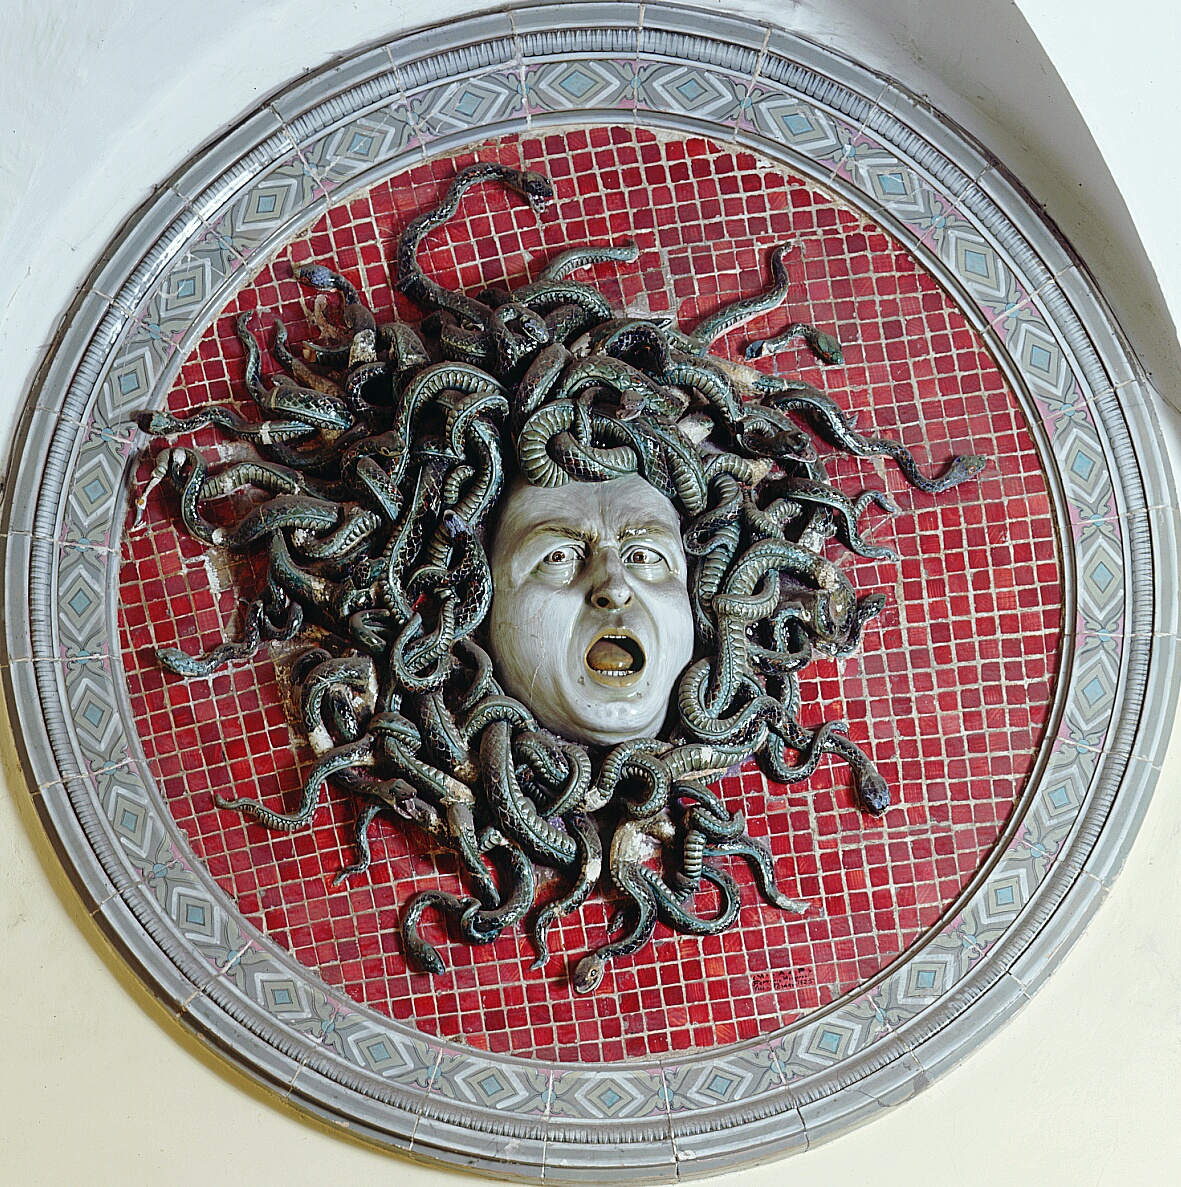
\includegraphics[scale=1]{Mengaroni_Ferruccio-Medusa.jpg}}
					};
				\end{tikzpicture}
				\captionsetup{labelformat=empty}
				\captionof{figure}{\#1}
				
			}&{}
		\end{tabularx}
	}
	
	% Second line
	\vspace{5mm}
	\nopagebreak
	\begin{tabularx}{\linewidth}{XX}
		{}&{
			% Bellini_Giovanni-Incoronazione_della_Vergine
			\begin{tikzpicture}
				\node[draw,dashed]
				{
					\setlength{\fboxsep}{0pt}\fbox{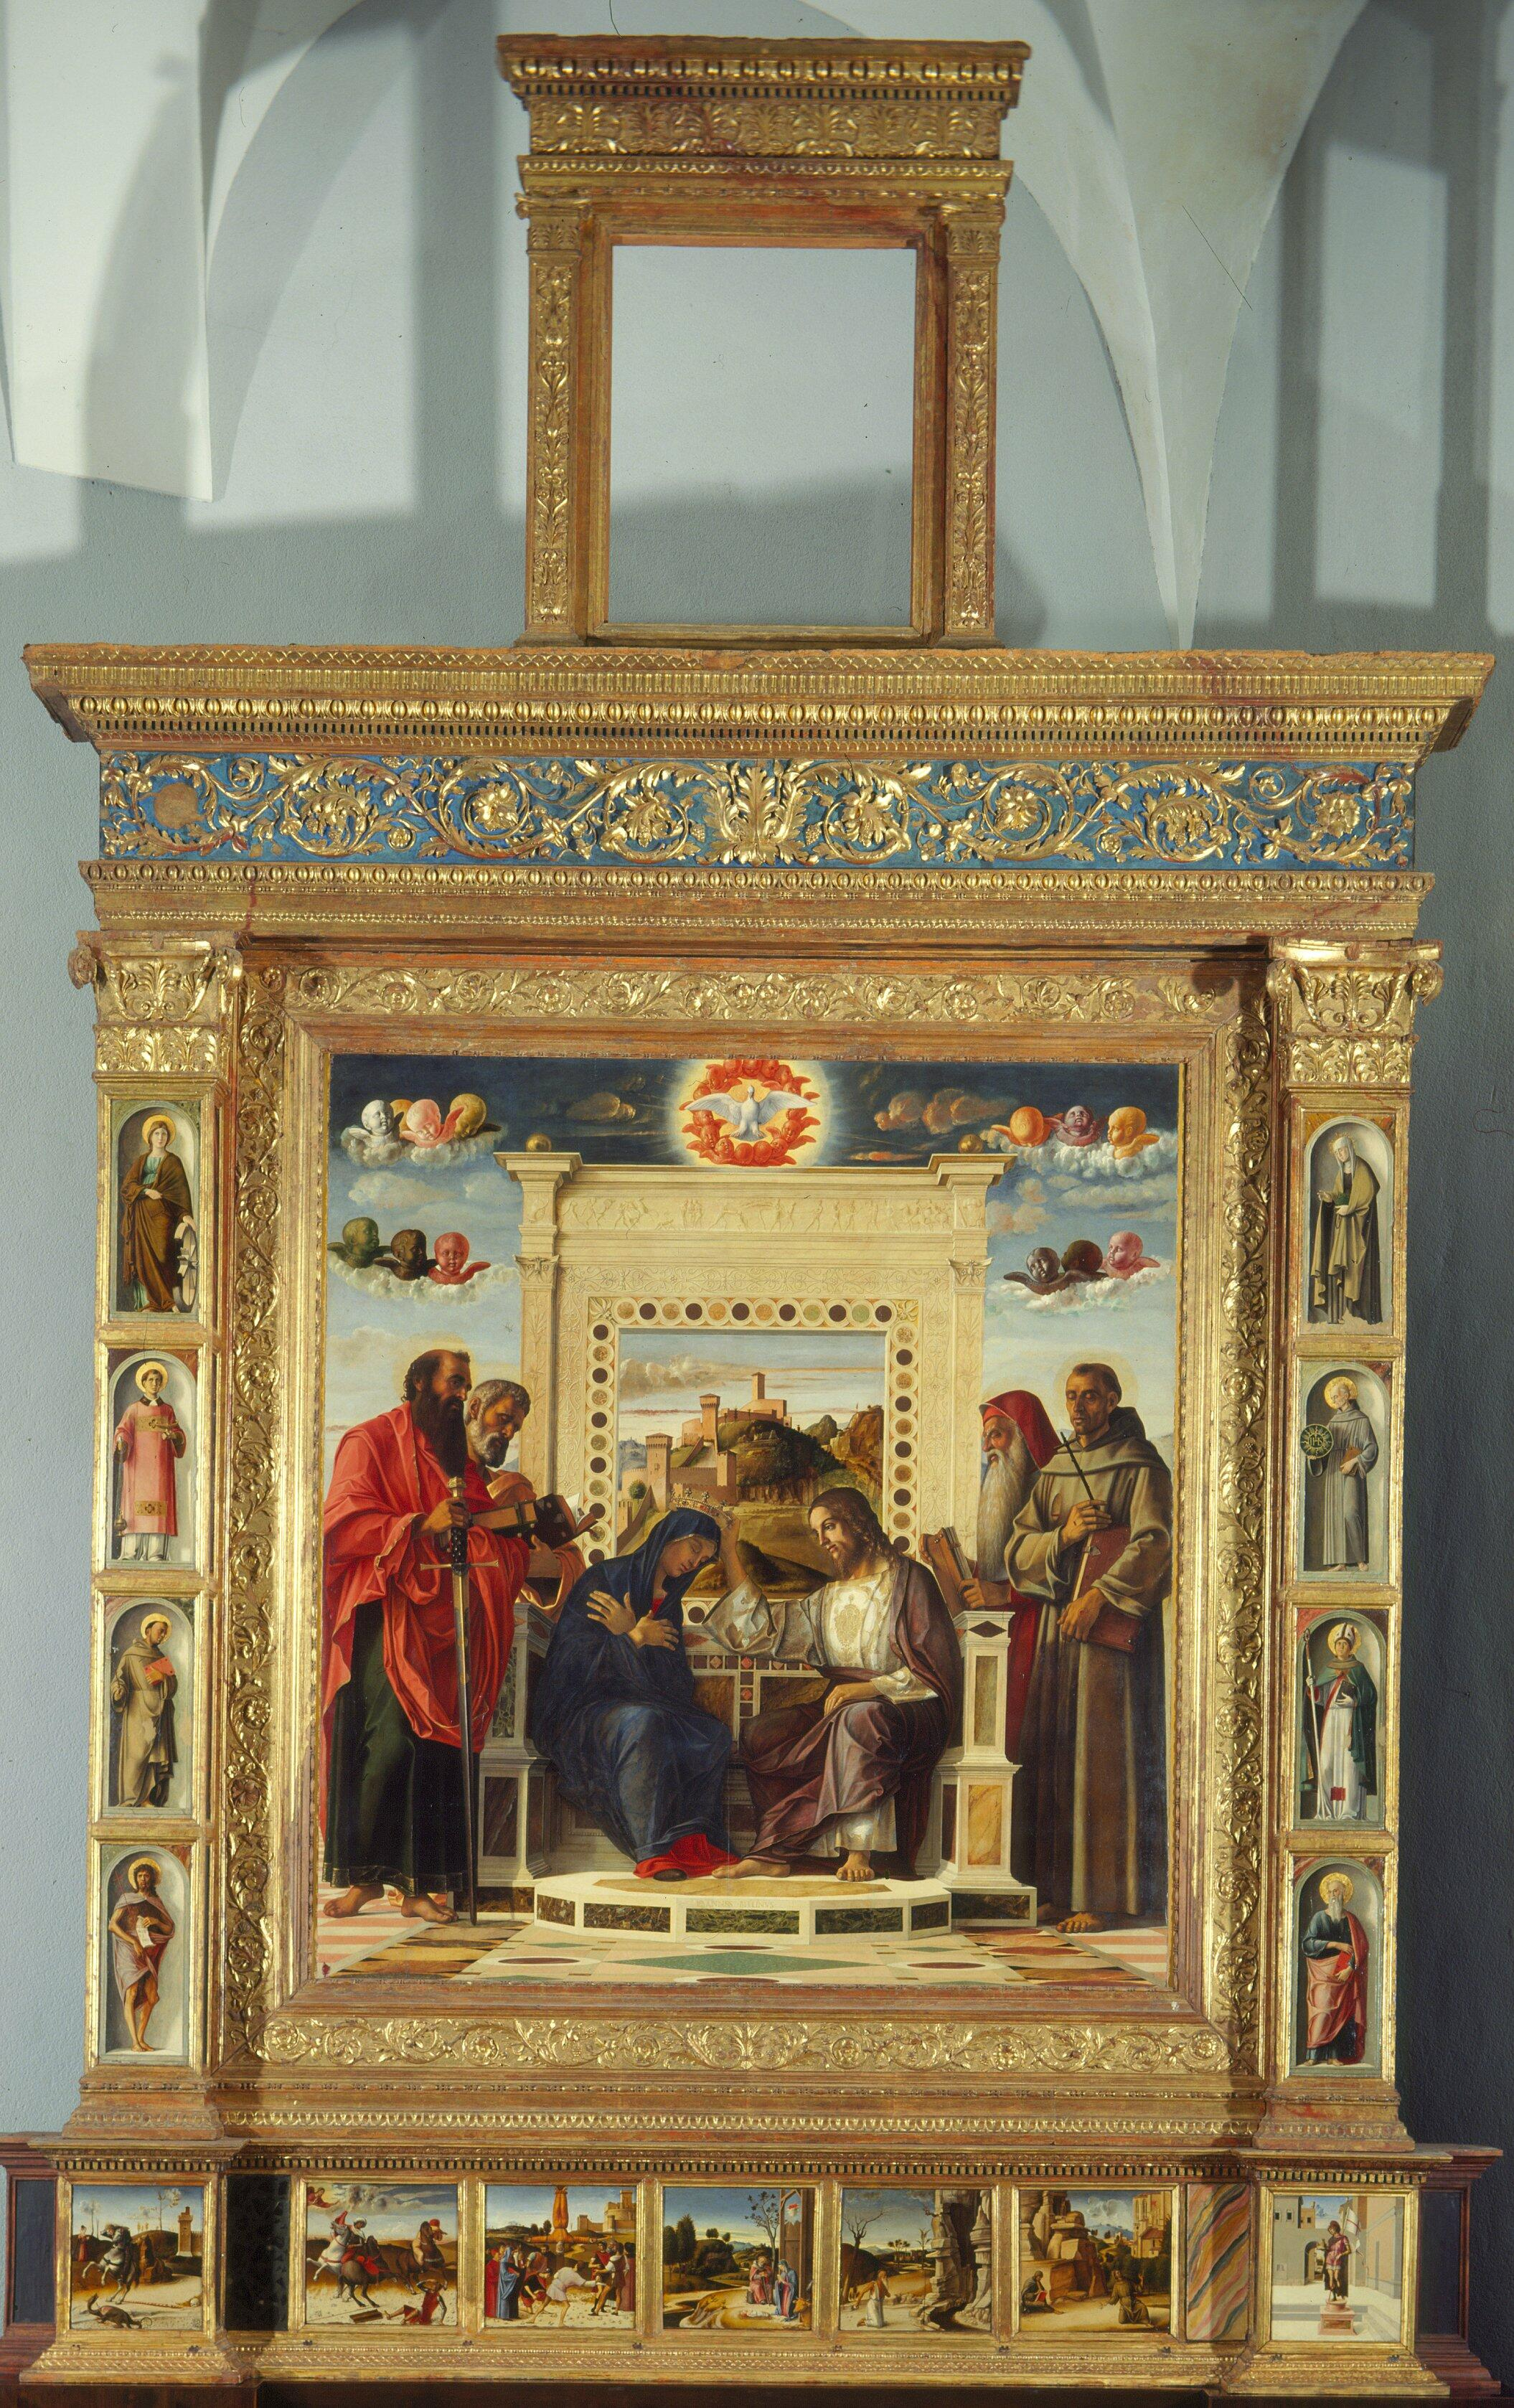
\includegraphics[scale=0.083]{Bellini_Giovanni-Incoronazione_della_Vergine.jpg}}
				};
			\end{tikzpicture}
			\captionsetup{labelformat=empty}
			\captionof{figure}{\#2}
		}
	\end{tabularx}
	
	\newpage
	
	%--------- Page 2 ----------
	
	% First line 
	\hspace{-40mm}{
	\begin{tabularx}{\textwidth}{XX}
		{
			\hspace{10mm}
			%Vitale da Bologna - Sant'Ambrogio in trono
			\begin{tikzpicture}
				\node[draw,dashed]
				{
					\setlength{\fboxsep}{0pt}\fbox{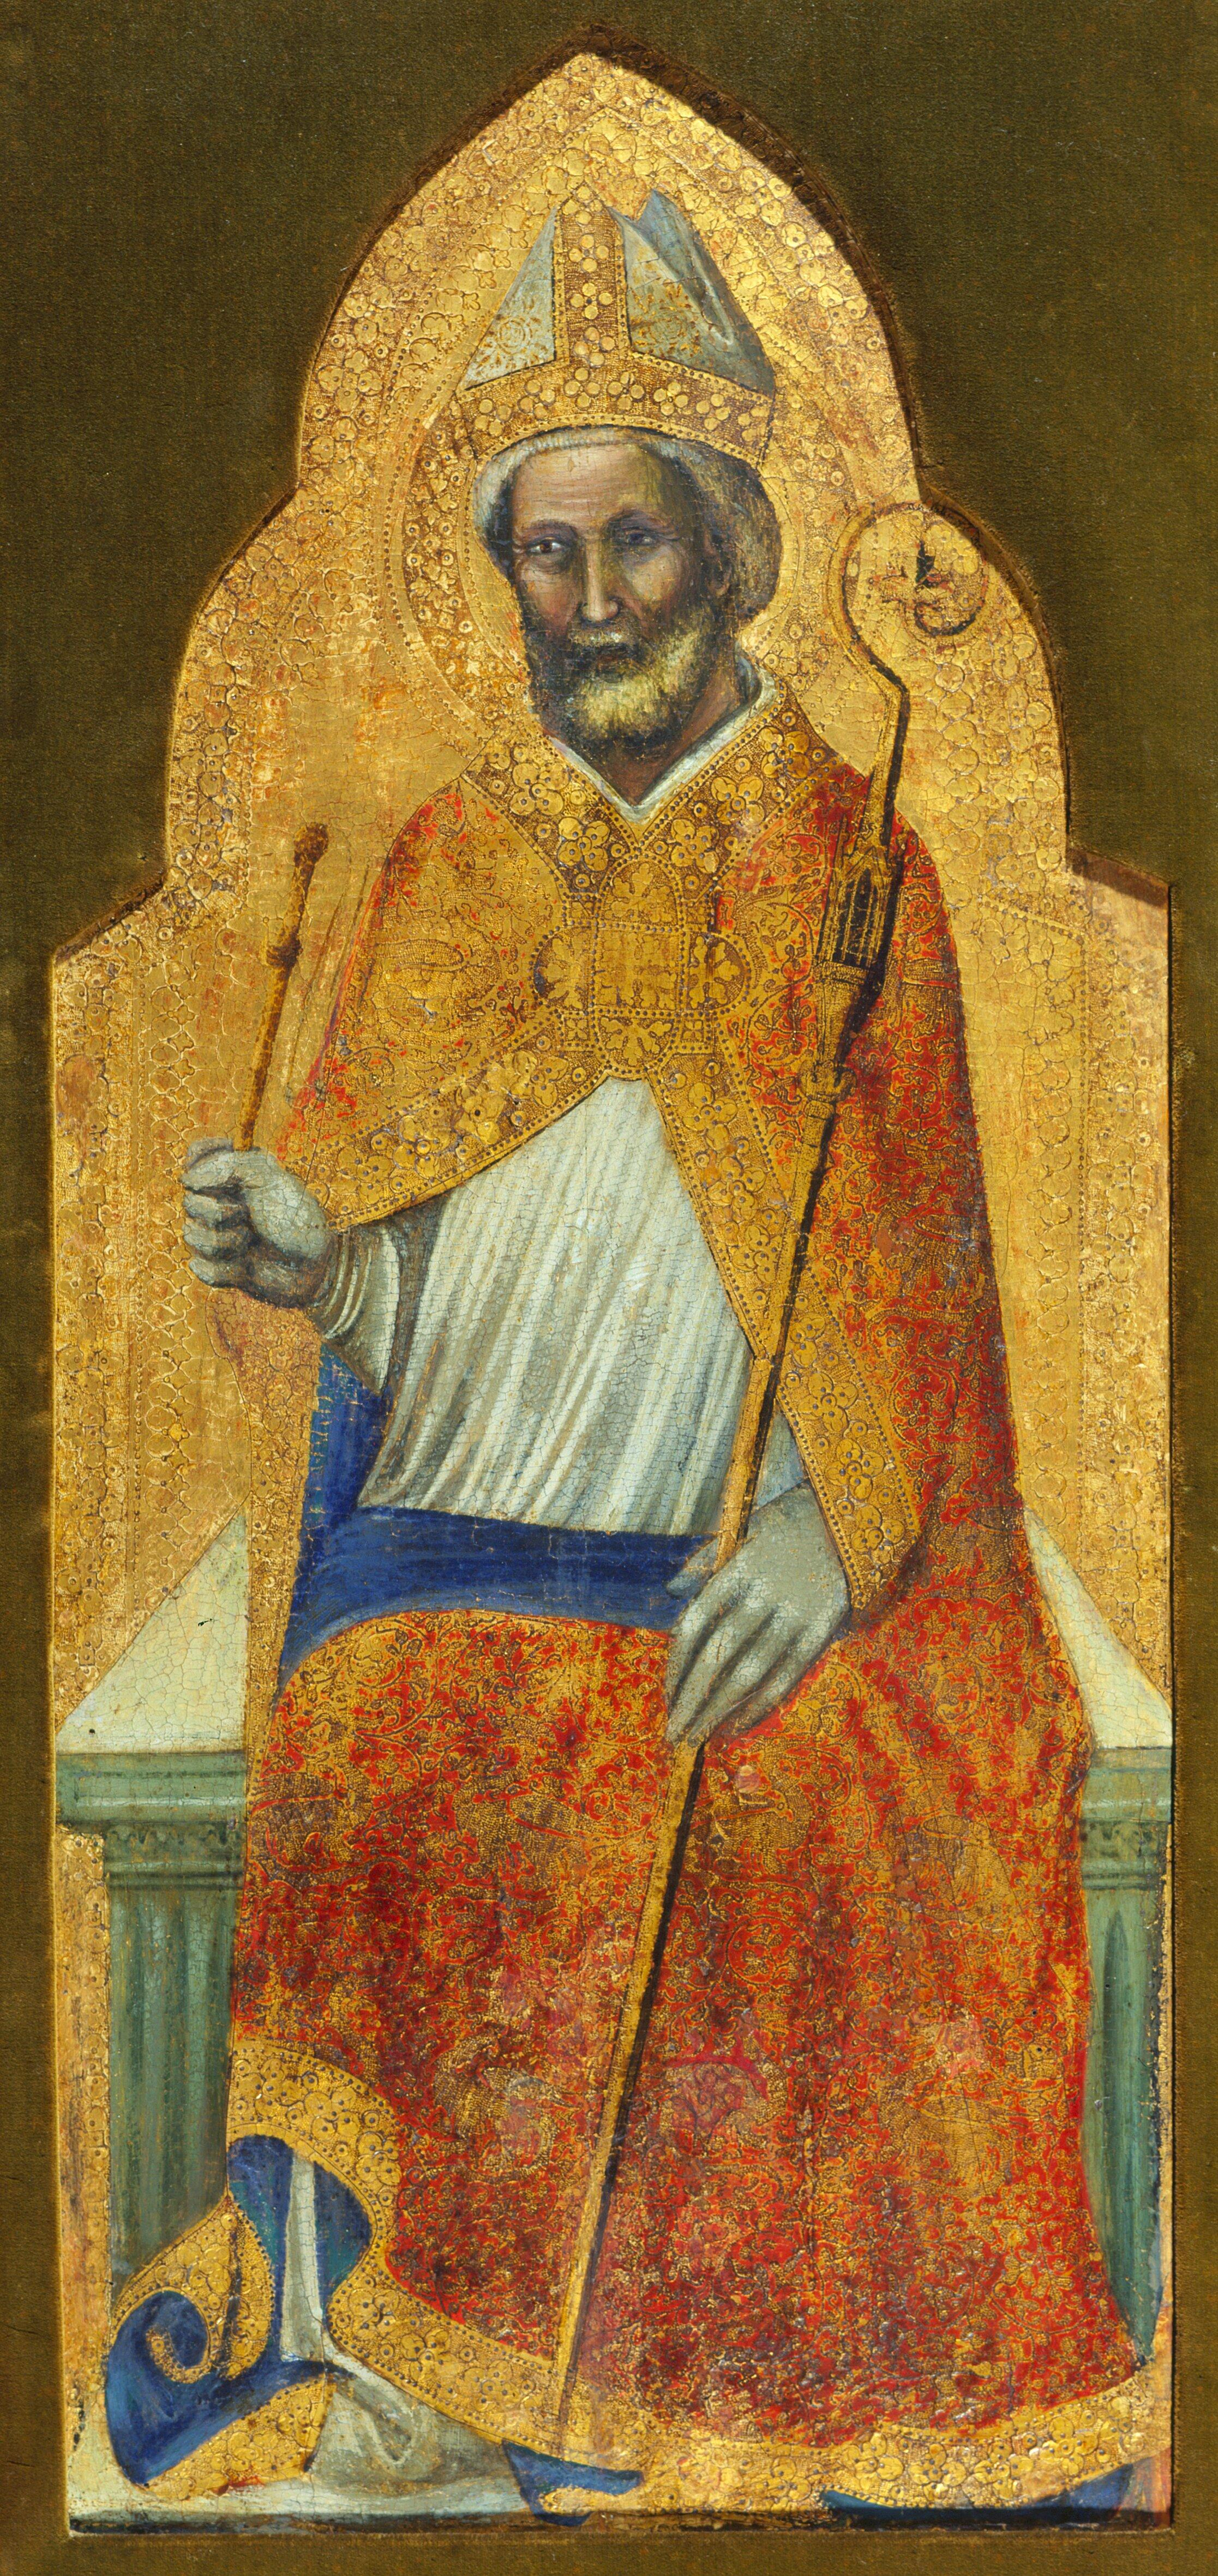
\includegraphics[scale=0.058]{Vitale_da_Bologna-Santo_Ambrogio_in_trono.jpg}}
				};
			\end{tikzpicture}
			\captionsetup{labelformat=empty}
			\captionof{figure}{\#3}
			
		}&{
			\hspace{20mm}{
			% Desani Pietro - Rebecca ed Eleazar
			\begin{tikzpicture}
				\node[draw,dashed]
				{
					\setlength{\fboxsep}{0pt}\fbox{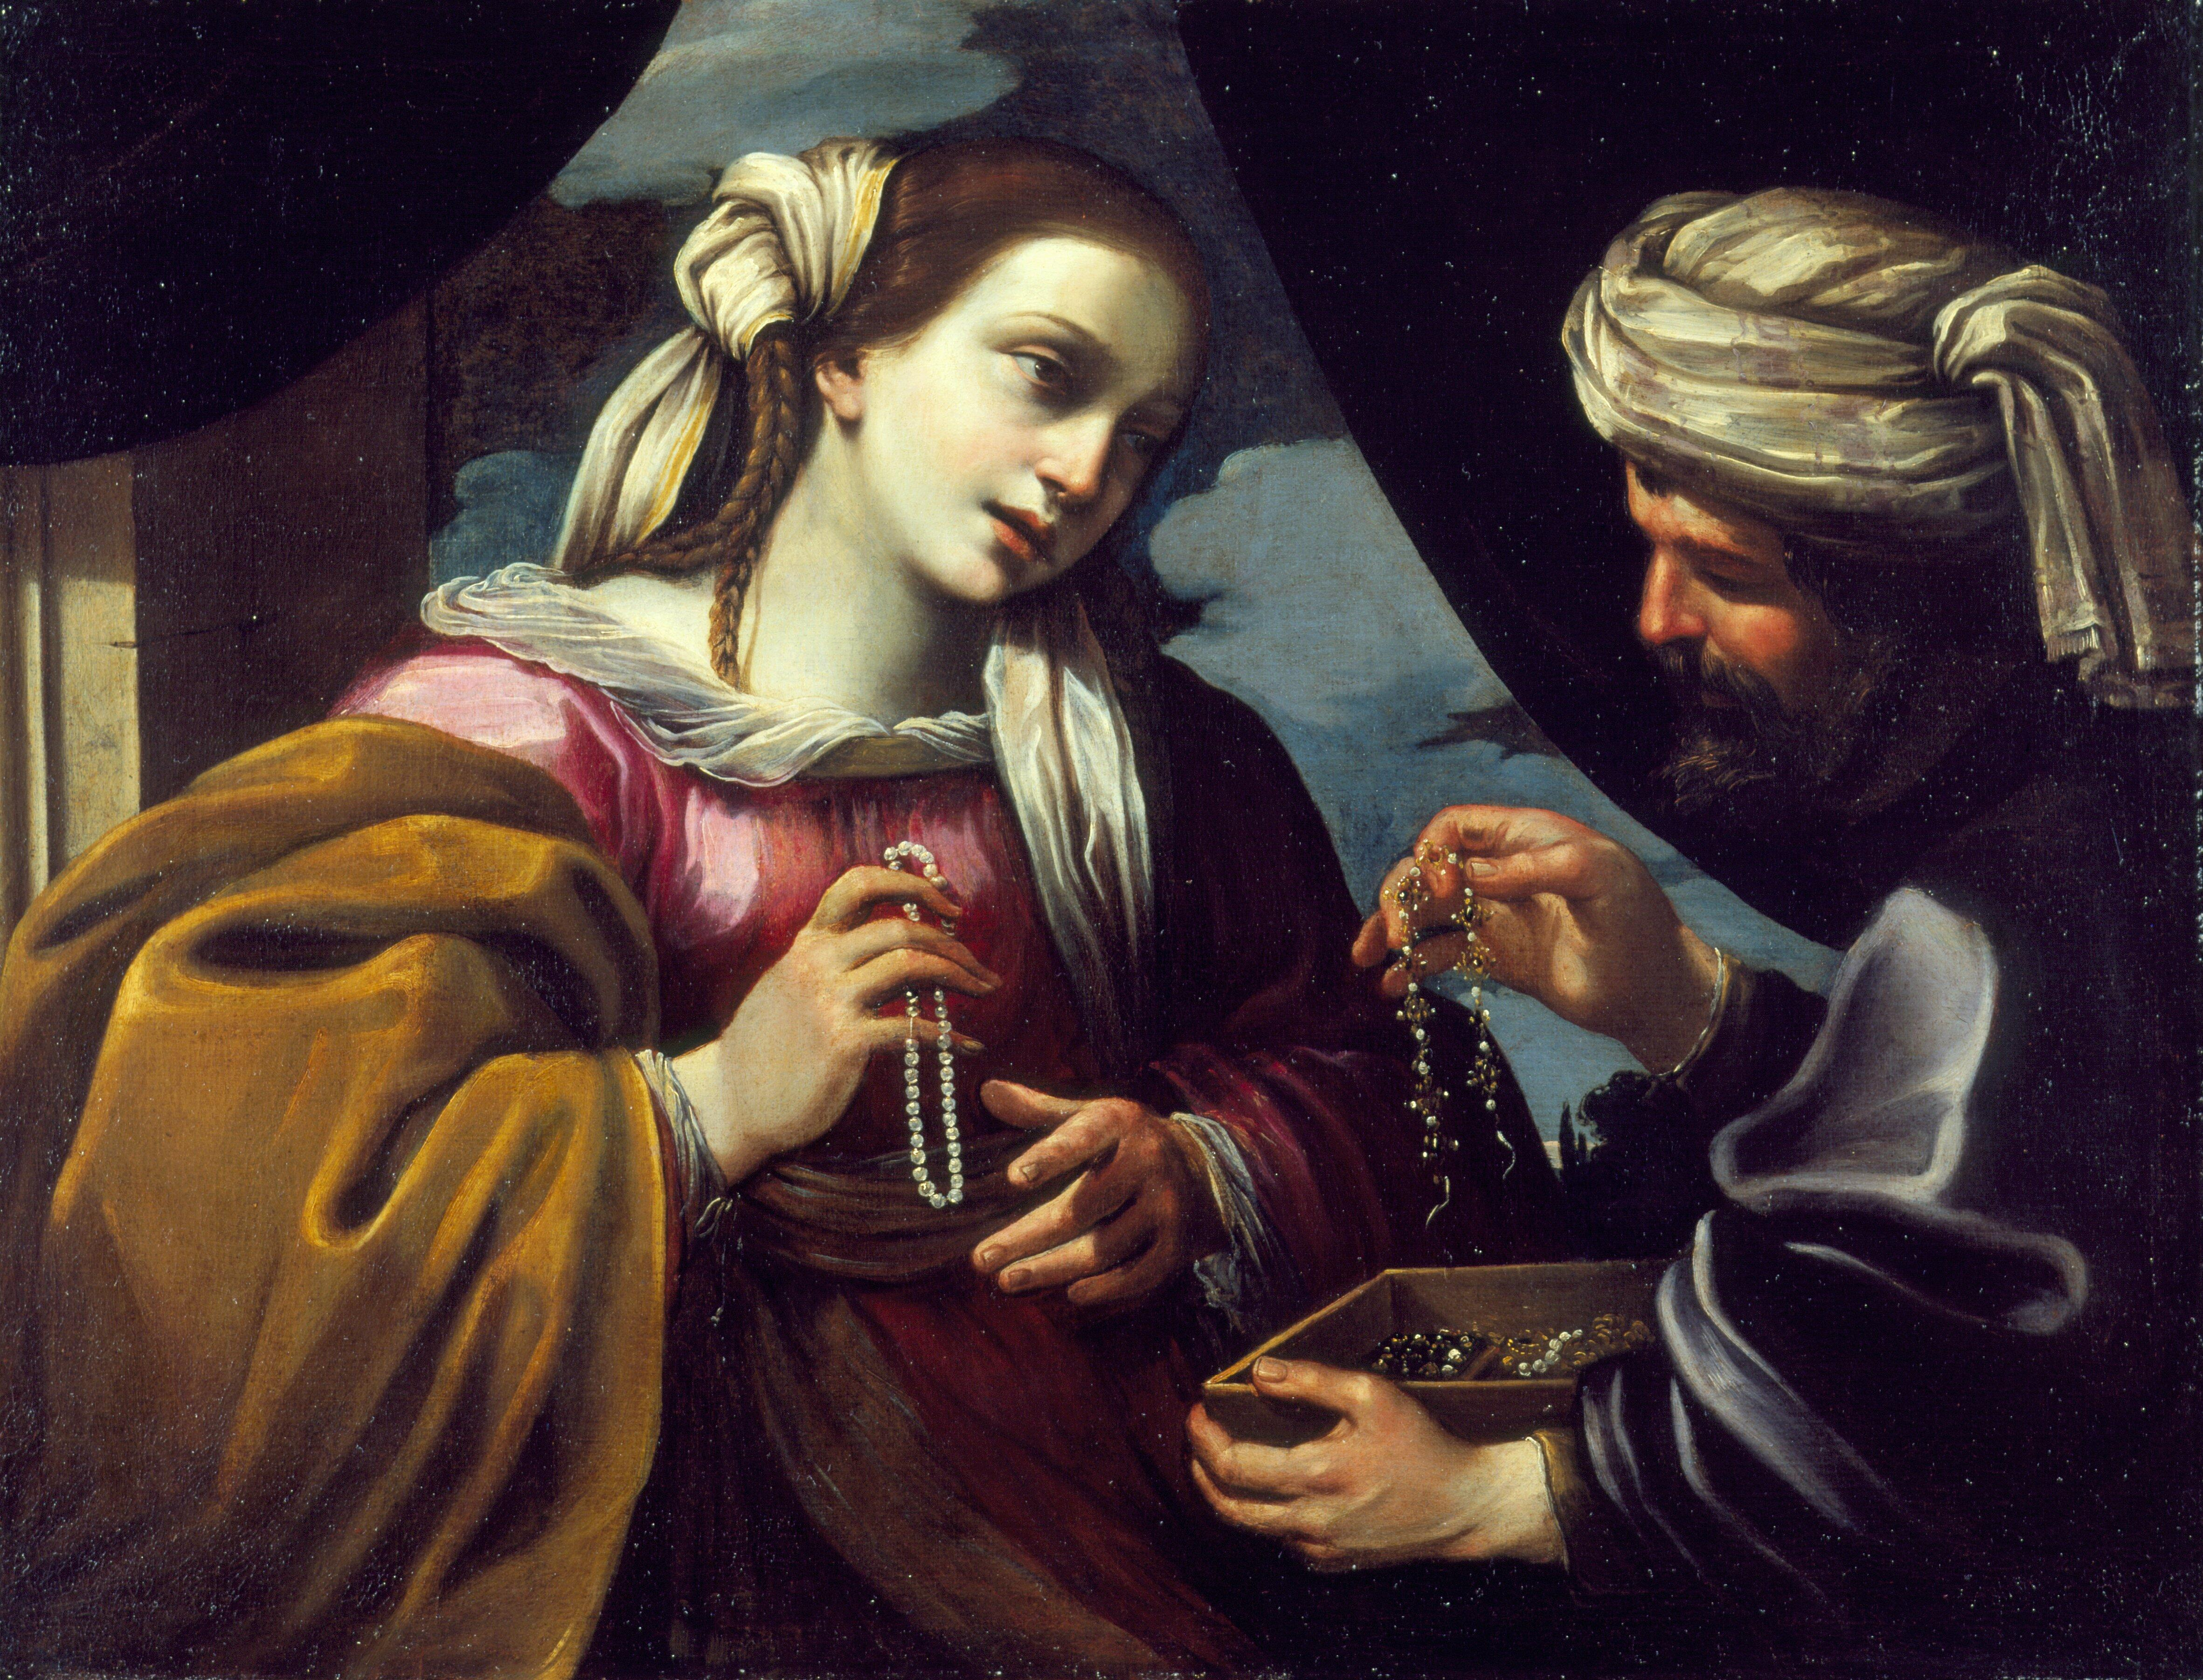
\includegraphics[scale = 0.048]{Desani_Pietro-Rebecca_ed_Eleazar.jpg}}
				};
			\end{tikzpicture}
				\captionsetup{labelformat=empty}
				\captionof{figure}{\hspace*{60mm}\#4}
			}
			
		}
	\end{tabularx}
	
	% Second line
	\nopagebreak
	\begin{tabularx}{\textwidth}{X}
		{	
			\begin{center}
				\hspace{27mm}
				%Giovanni Antonio Garella - Leda e il cigno
				\begin{tikzpicture}
					\node[draw,dashed]
					{
						\setlength{\fboxsep}{0pt}\fbox{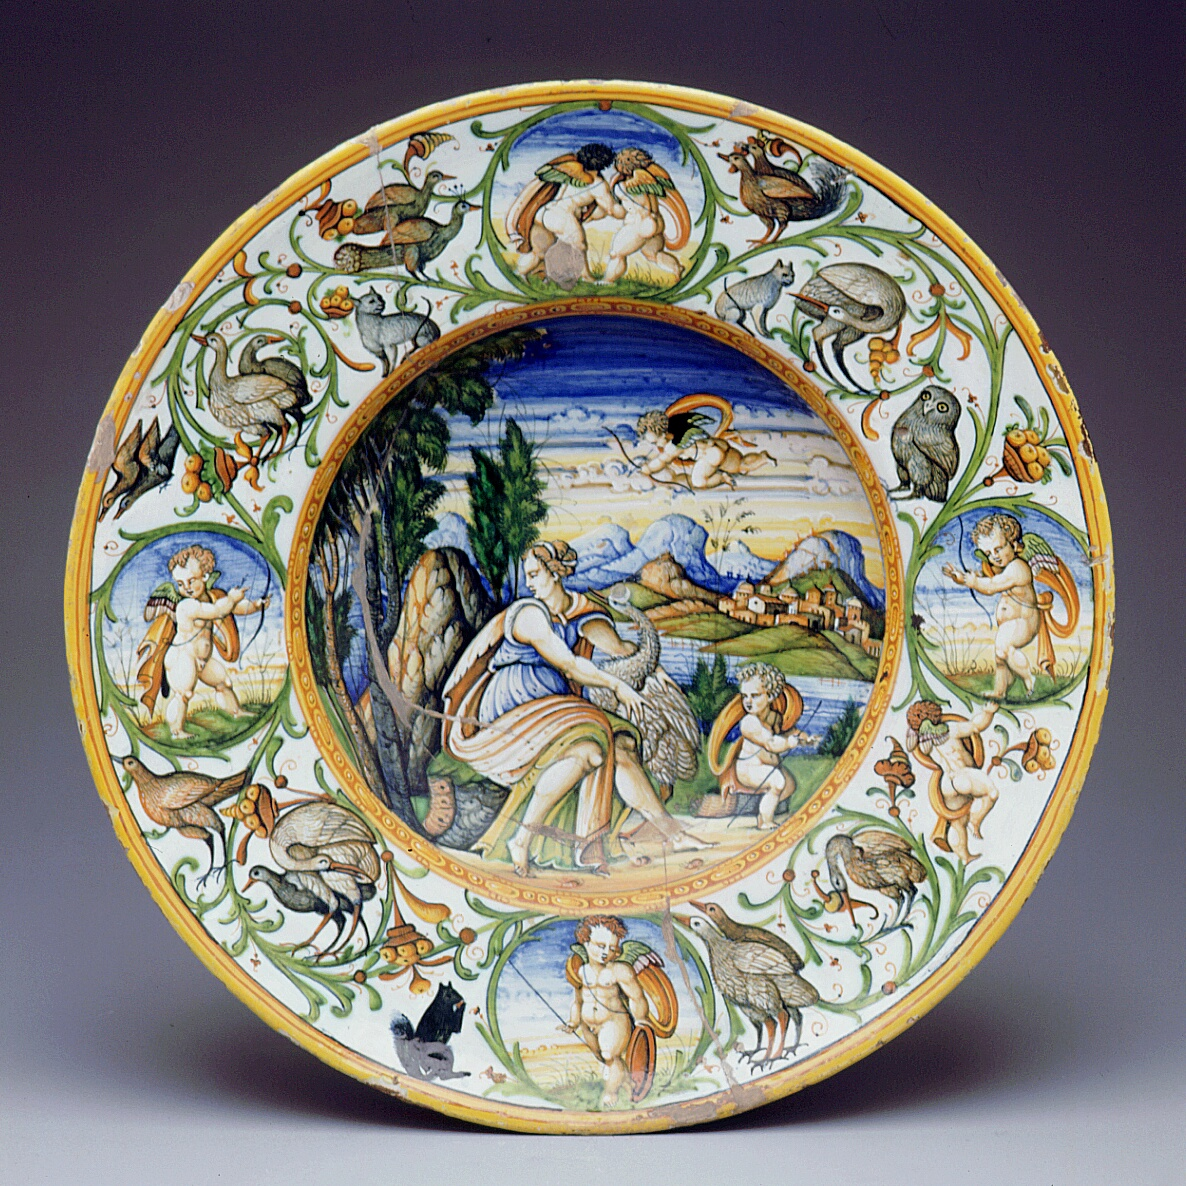
\includegraphics[scale=0.98]{Giovanni_Antonio_Garella-Leda_e_il_cigno.jpg}}
					};
				\end{tikzpicture}
				\captionsetup{labelformat=empty}
				\captionof{figure}{\hspace*{30mm}\#5}
			\end{center}
		}
	\end{tabularx}
	
	\newpage
	
	%--------- Page 3 ----------
	
	% First line 
	\vspace*{-10mm}
	\begin{tabularx}{\textwidth}{XX}
		{
			\begin{center}
				\hspace{5mm}
				%Specchio in vetro di Murano
				\begin{tikzpicture}
					\node[draw,dashed]
					{
						\setlength{\fboxsep}{0pt}\fbox{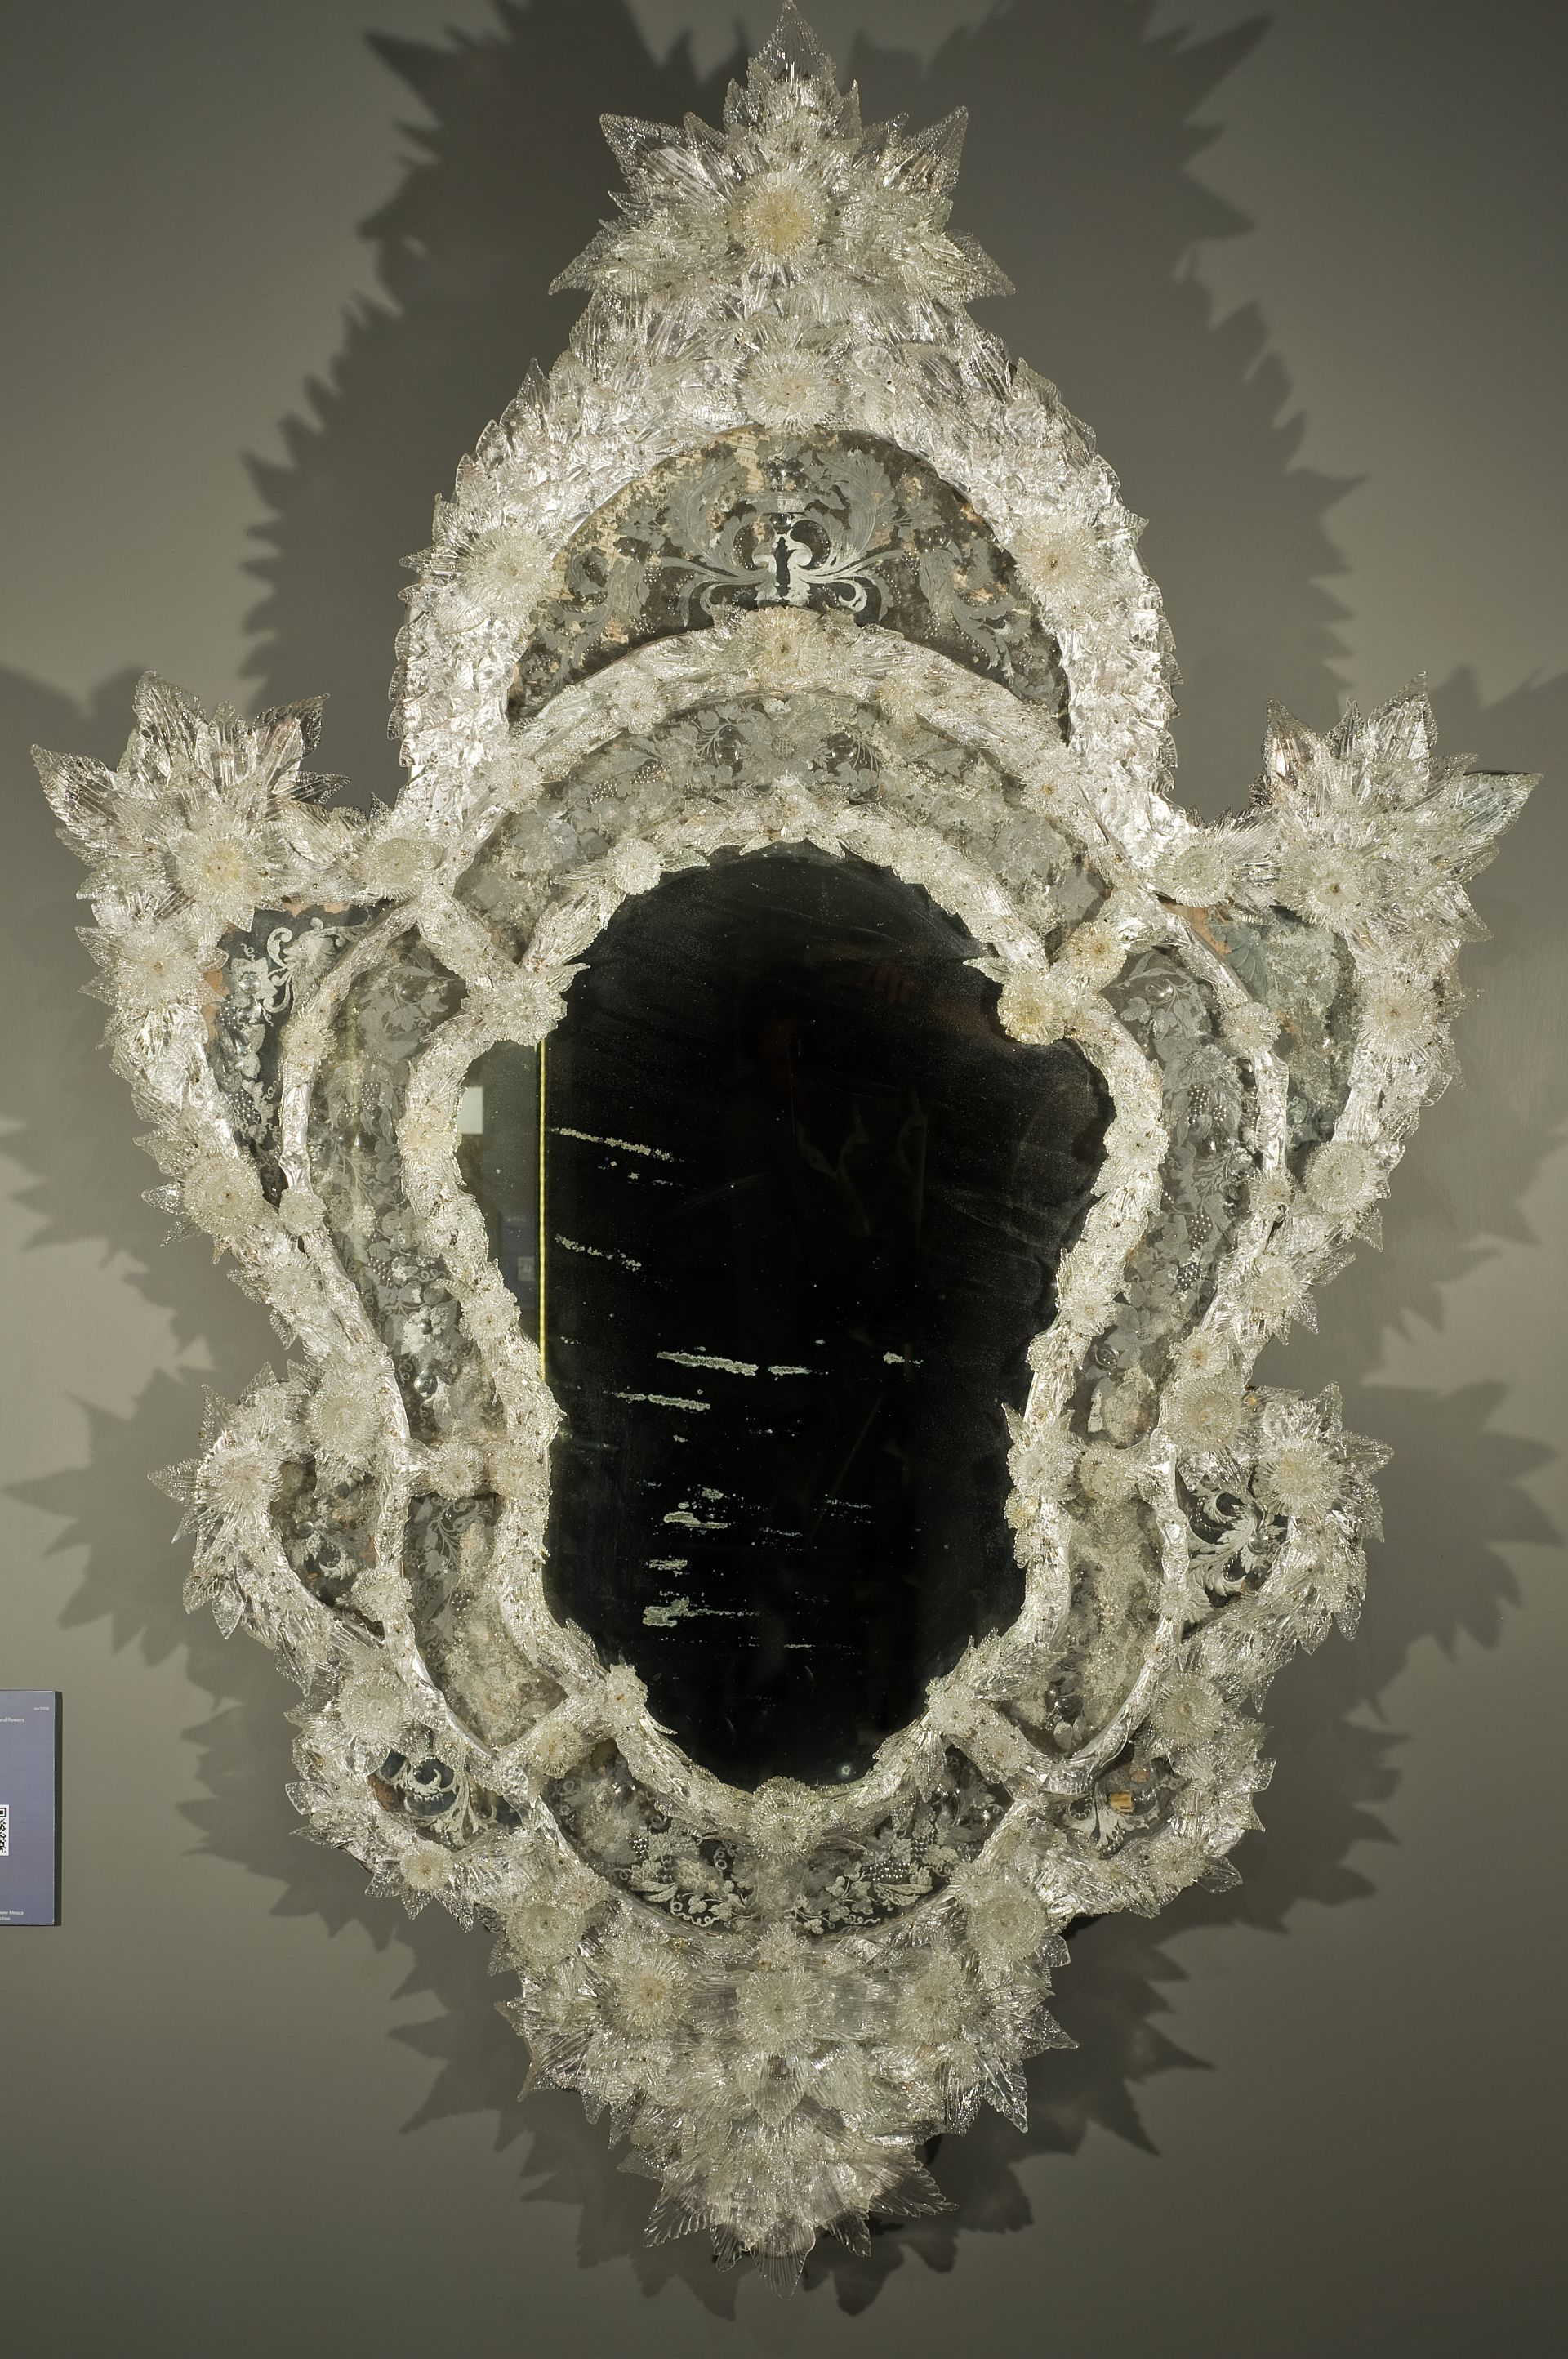
\includegraphics[scale=0.28]{Specchio_di_Murano.jpg}}
					};
				\end{tikzpicture}
				\captionsetup{labelformat=empty}
				\captionof{figure}{\#6}
			\end{center}
		}&{
			\vspace{20mm}
			%Vedute di Roma
			\hspace{10mm}{
				\begin{tikzpicture}
					\node[draw,dashed]
					{
						\setlength{\fboxsep}{0pt}\fbox{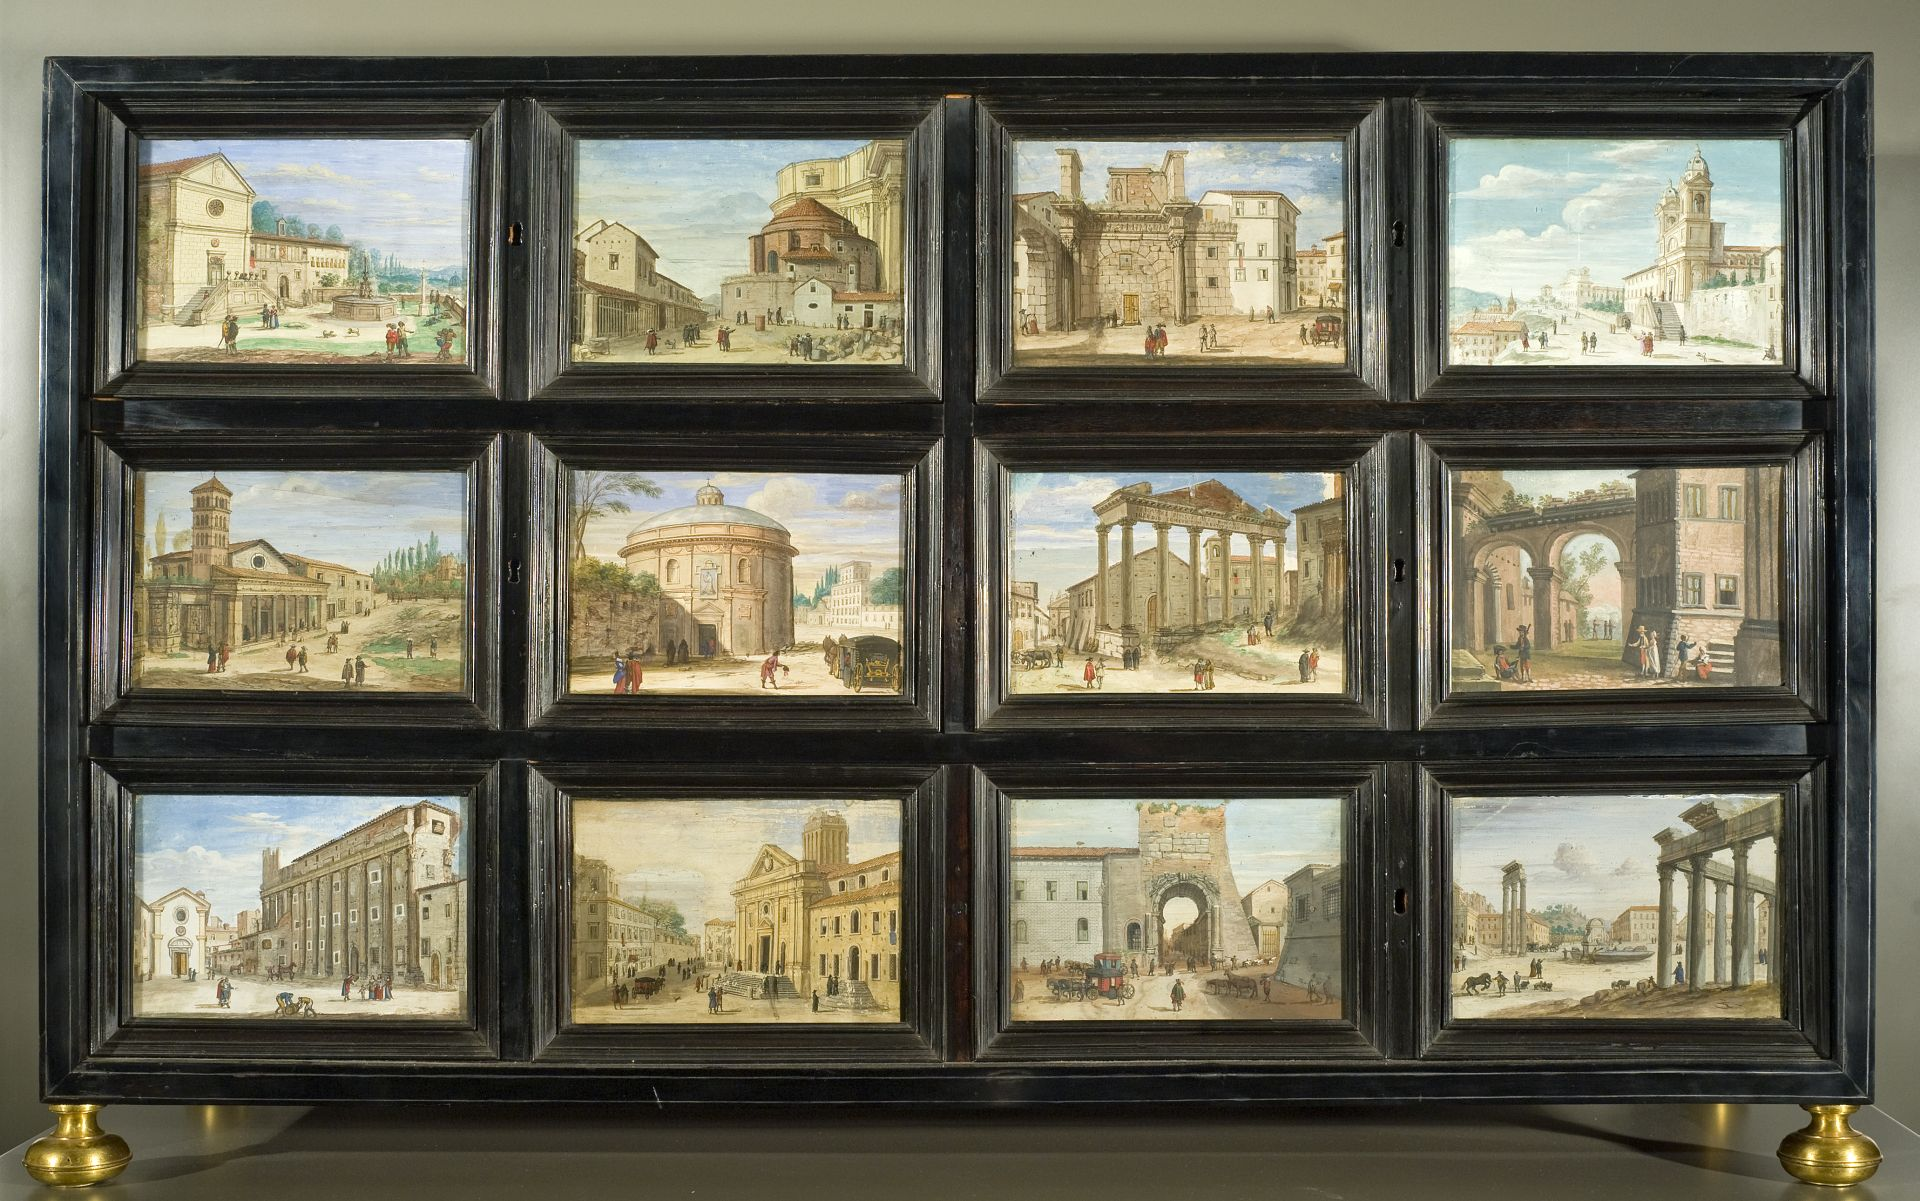
\includegraphics[scale=0.33]{Vedute_di_Roma_1.jpg}}
					};
				\end{tikzpicture}
				\captionsetup{labelformat=empty}
				\captionof{figure}{\hspace*{30mm}\#7}
			}
		}
	\end{tabularx}
	
	% Second line
	\nopagebreak
	\begin{tabularx}{\linewidth}{XX}
		{}&{
			\hspace{15mm}
			\begin{tikzpicture}
				\node[draw,dashed]
				{
					\setlength{\fboxsep}{0pt}\fbox{\includegraphics[scale=0.18]{Orologio_notturno.jpg}}
				};
			\end{tikzpicture}
			\captionsetup{labelformat=empty}
			\captionof{figure}{\hspace*{20mm}\#8}
		}
	\end{tabularx}
	
	\newpage
	
	%--------- Page 4 ----------
	
	% First line
	\vspace*{-30mm}
		\begin{tabularx}{\linewidth}{XX}
			{		
				\hspace{5mm}
				%Milani Aureliano - Mercato
				\begin{tikzpicture}
					\node[draw,dashed]
					{
						\setlength{\fboxsep}{0pt}\fbox{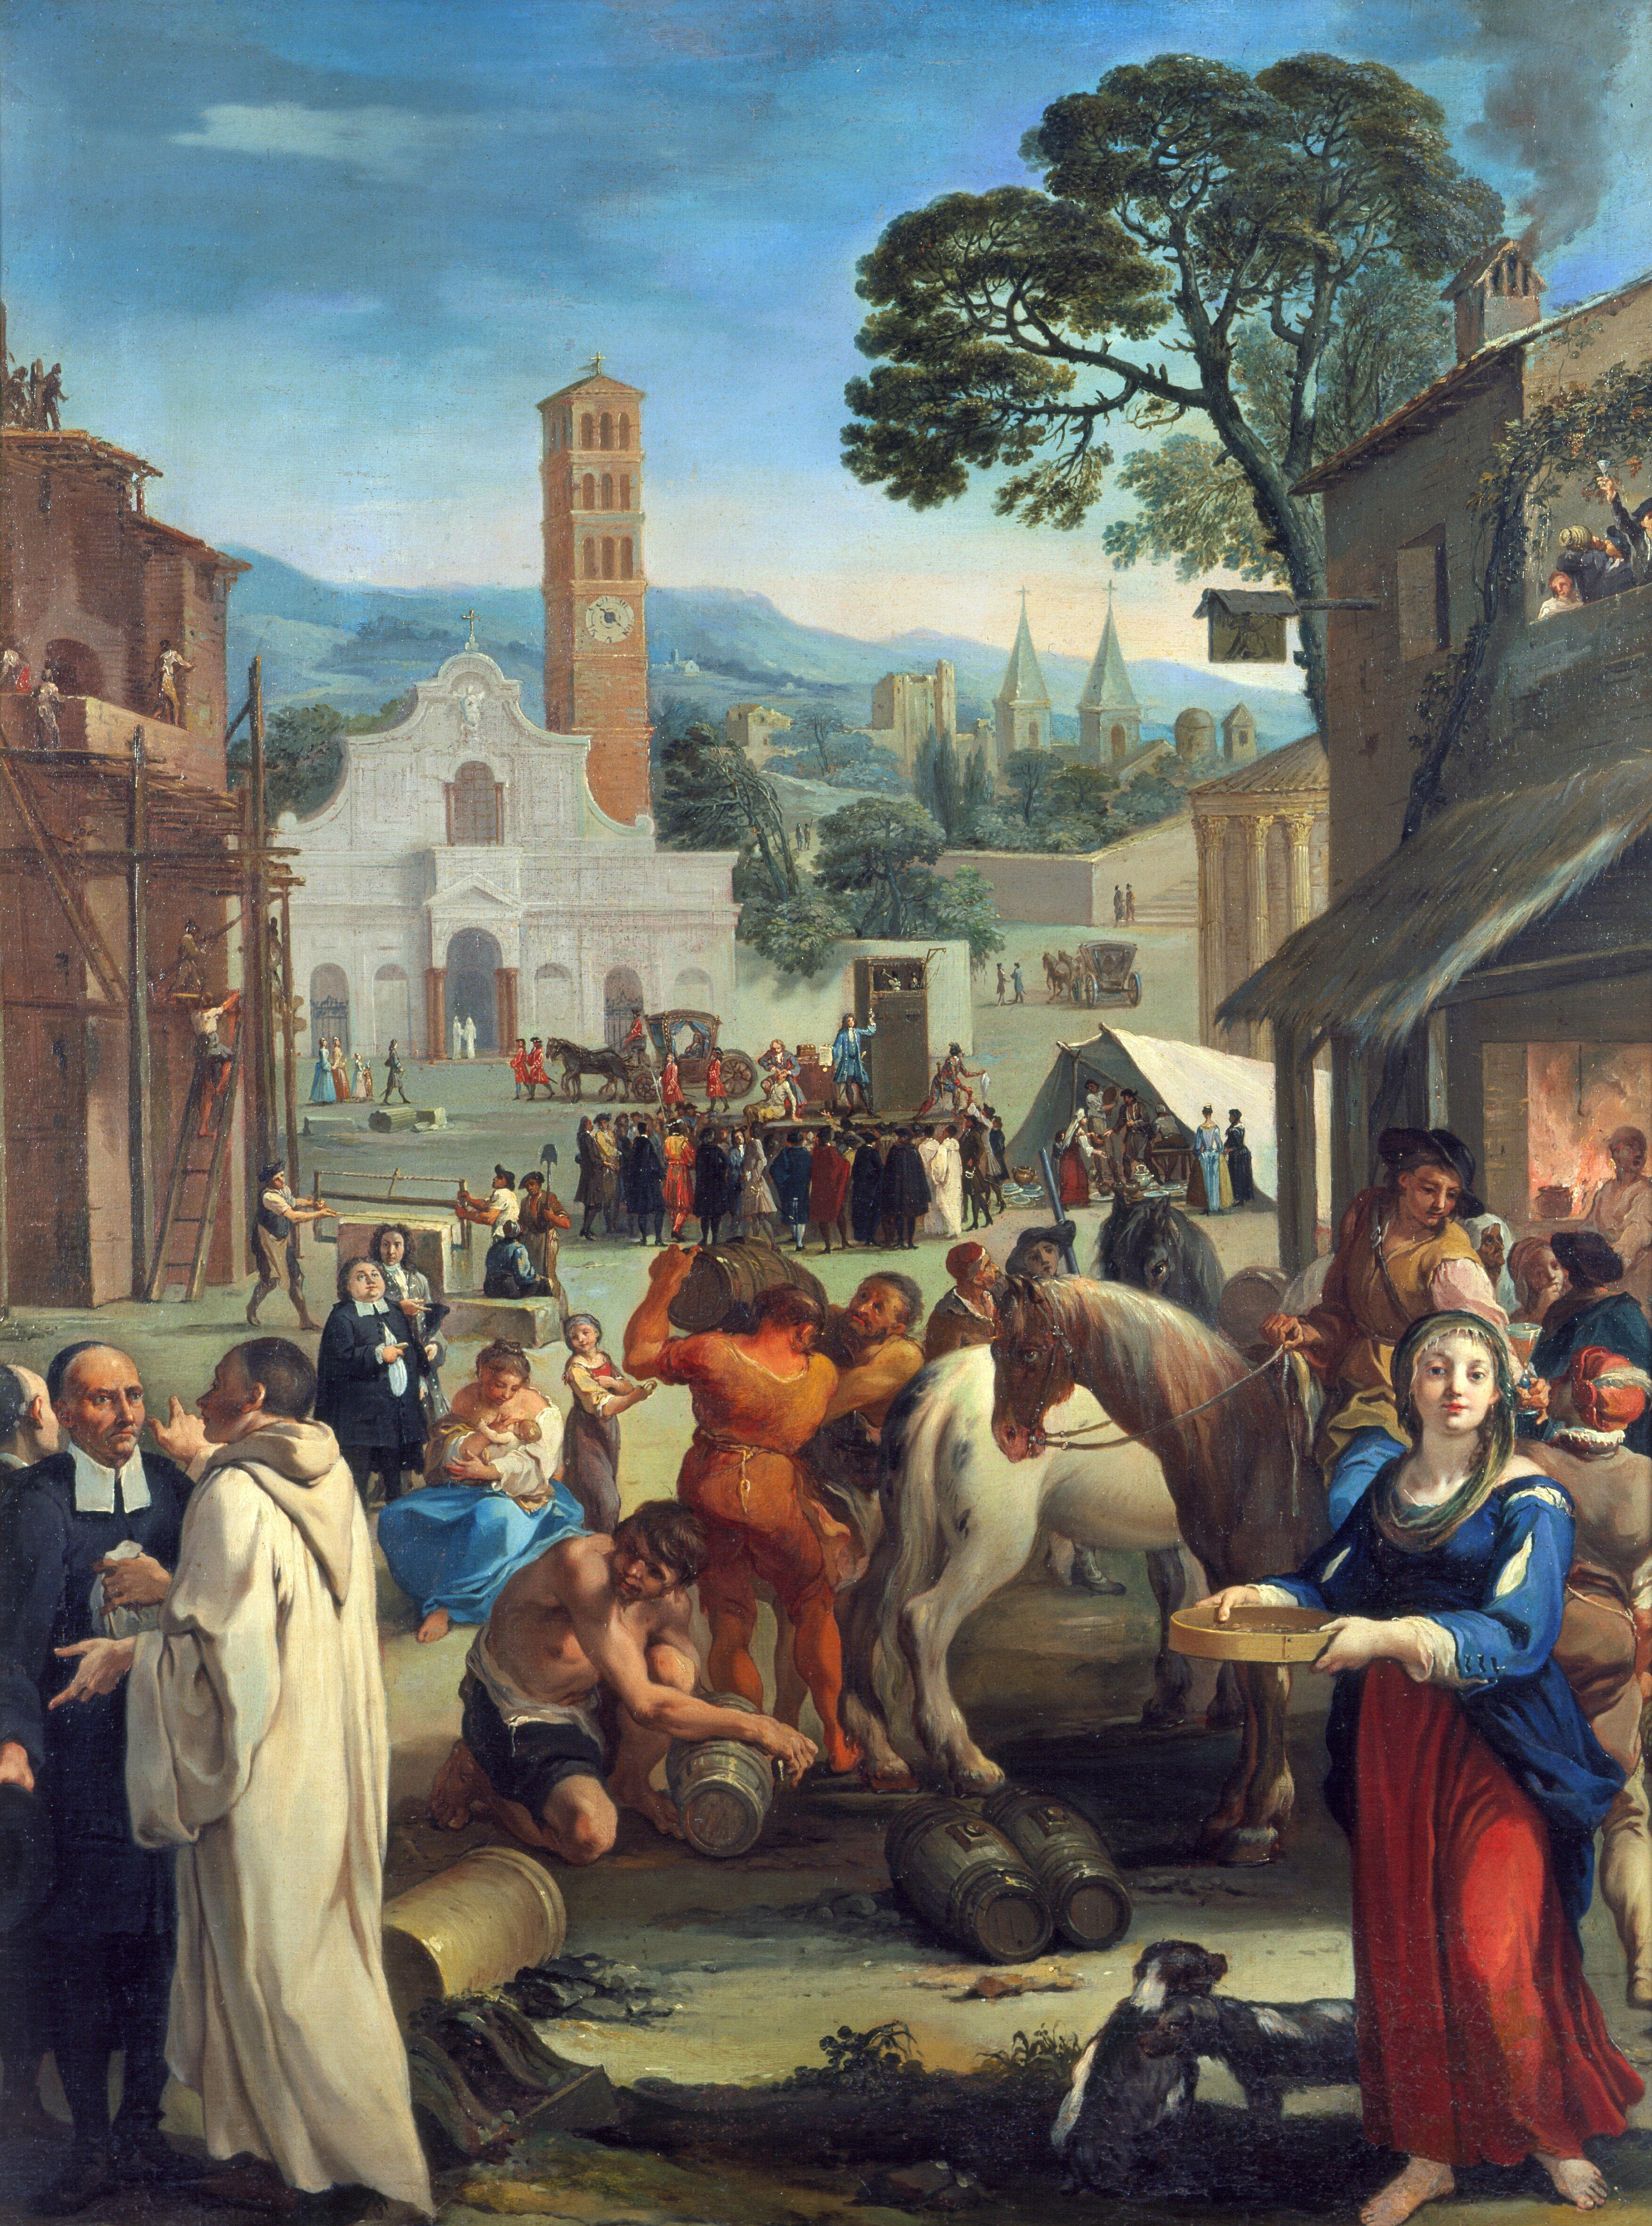
\includegraphics[scale=0.047]{Milani_Aureliano-Mercato.jpg}}
					};
				\end{tikzpicture}
				\captionsetup{labelformat=empty}
				\captionof{figure}{\hspace*{10mm}\#9}
				
			}&{
				\hspace{3mm}
				%Berentz Christian - Fiori e frutta con bicchieri di cristallo
				\begin{tikzpicture}
					\node[draw,dashed]
					{
						\setlength{\fboxsep}{0pt}\fbox{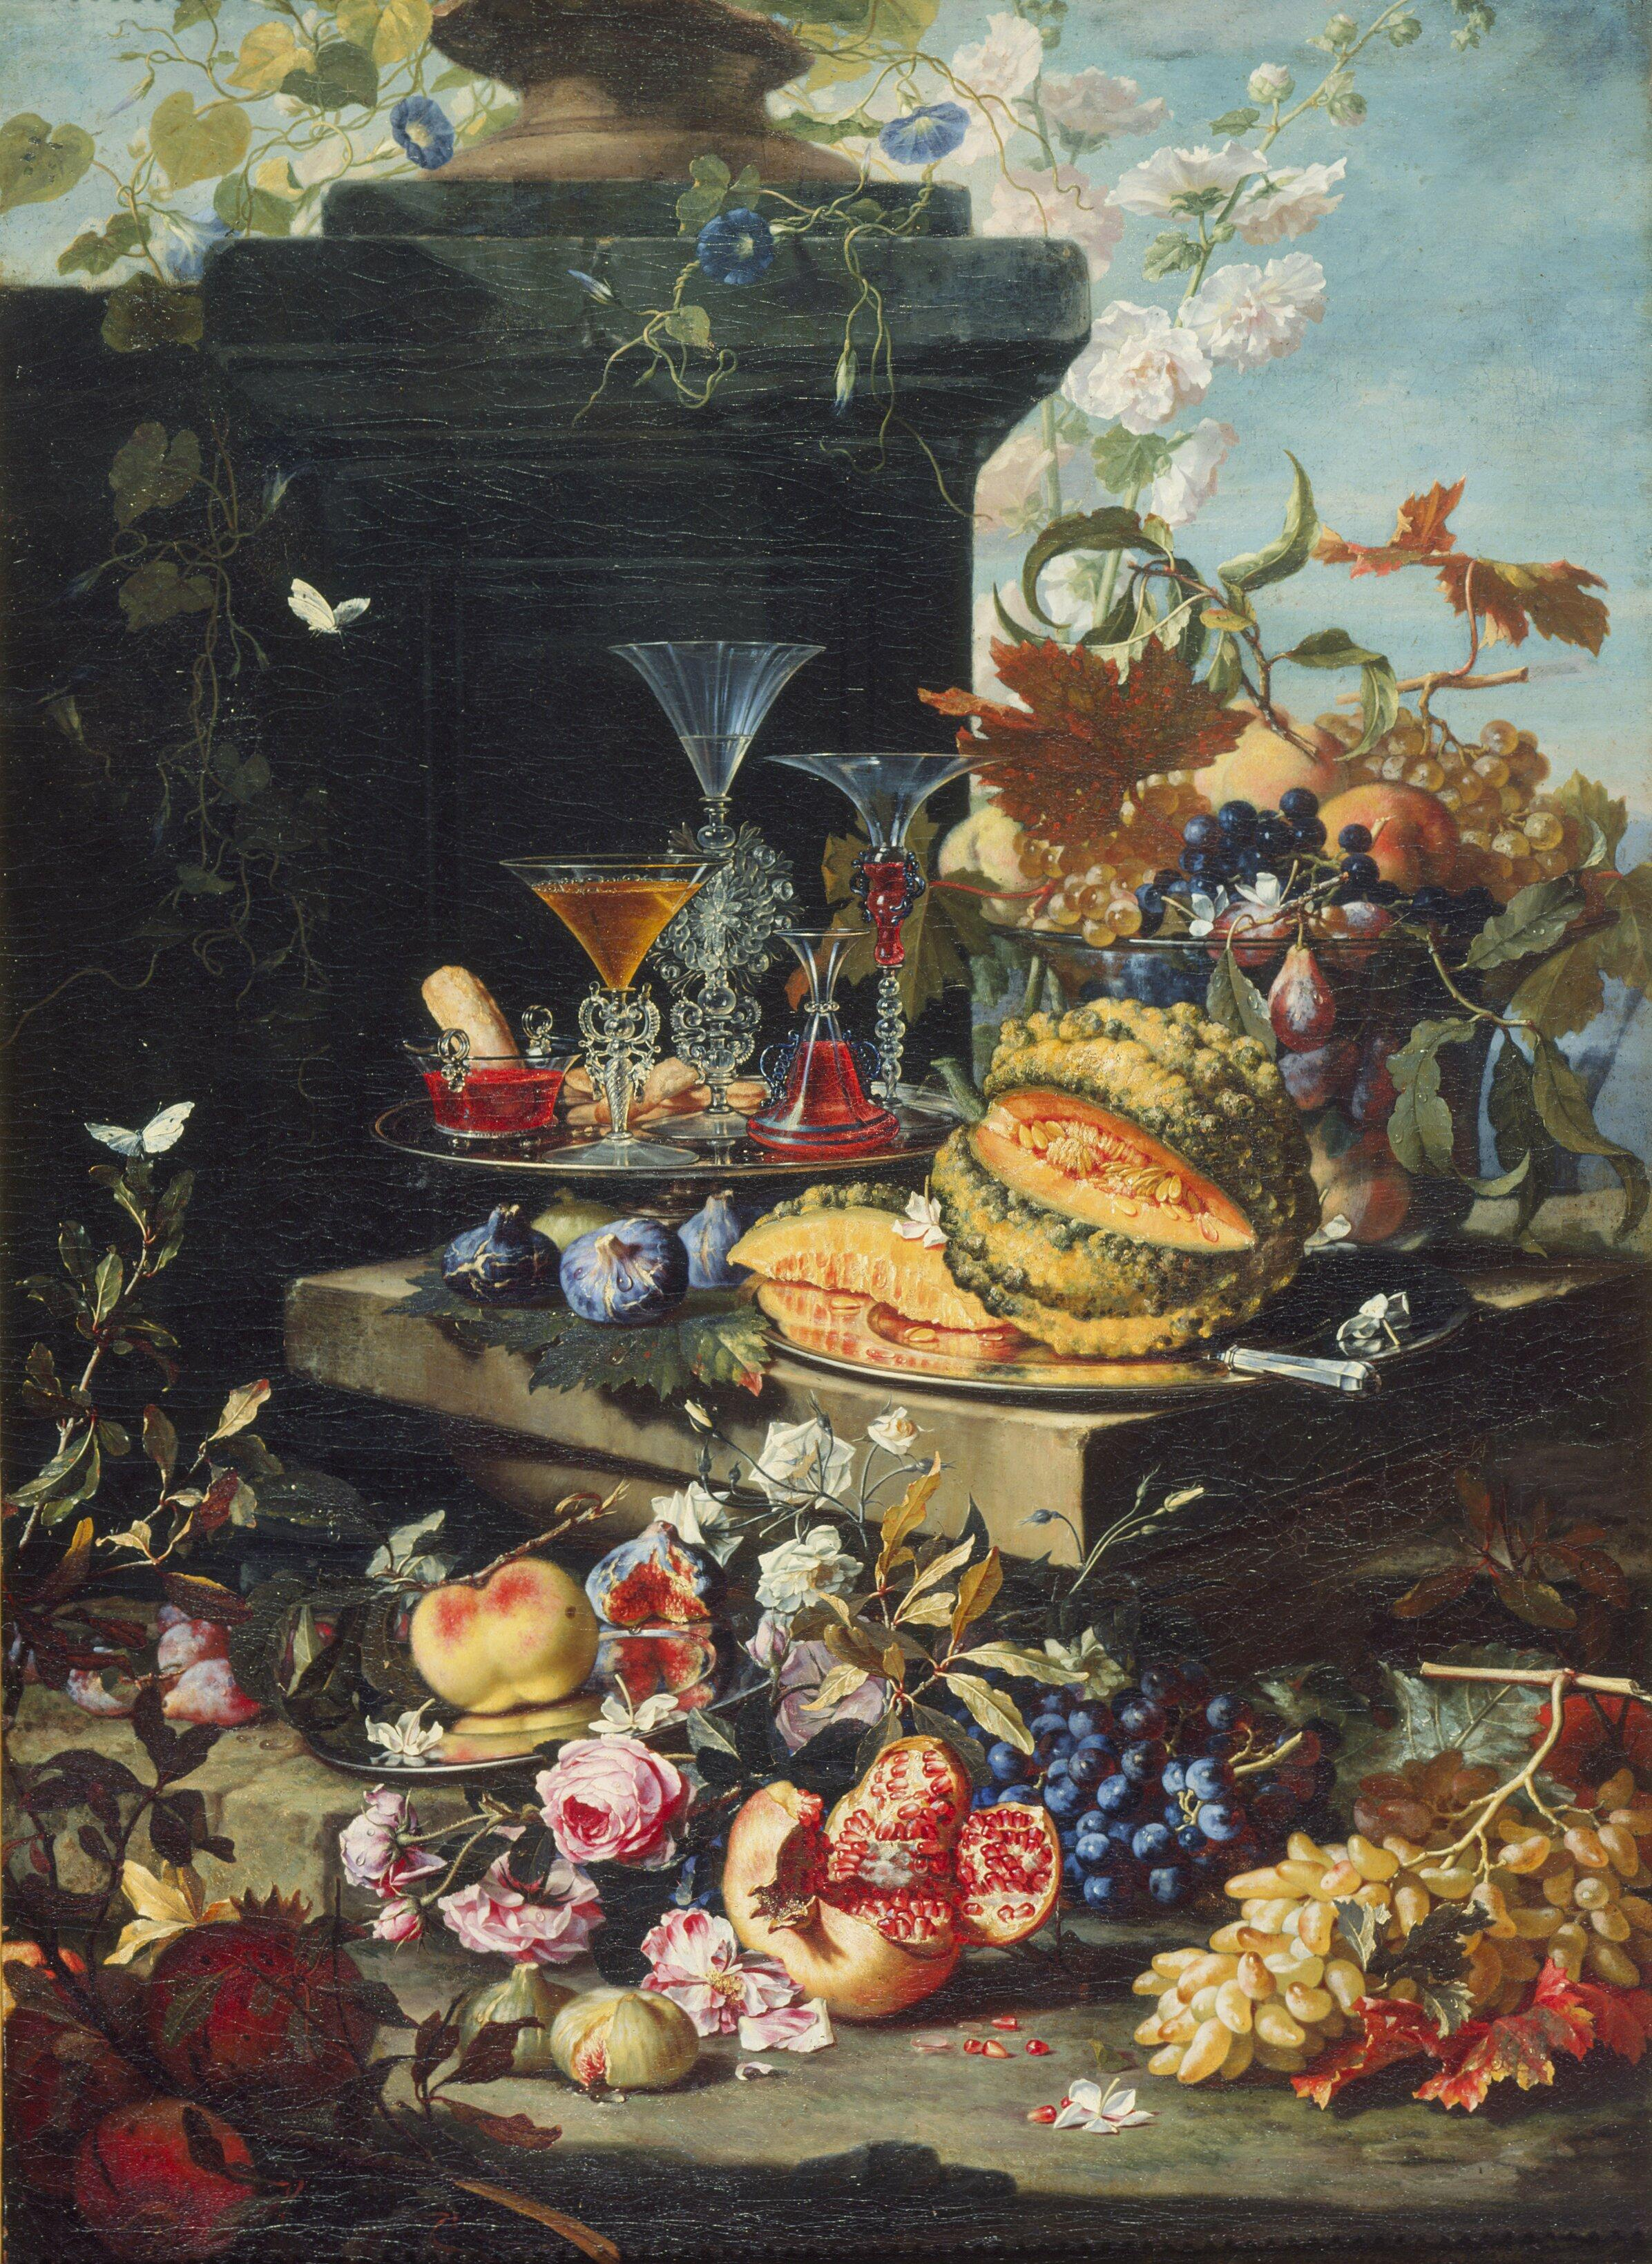
\includegraphics[scale= 0.078]{Berentz_Christian-Fiori_e_frutta_con_bicchieri_di_cristallo.jpg}}
					};
				\end{tikzpicture}
				\captionsetup{labelformat=empty}
				\captionof{figure}{\hspace*{10mm}\#10}
				
			}
		\end{tabularx}
	
		\nopagebreak
		\begin{tabularx}{\linewidth}{XX}
			{	
				\hspace{5mm}	
				%Gianlisi Antonio Junior - Trompe l'oeil con sonetto in onore di Eugenio di Savoia e mensola con oggetti
				\begin{tikzpicture}
					\node[draw,dashed]
					{
						\setlength{\fboxsep}{0pt}\fbox{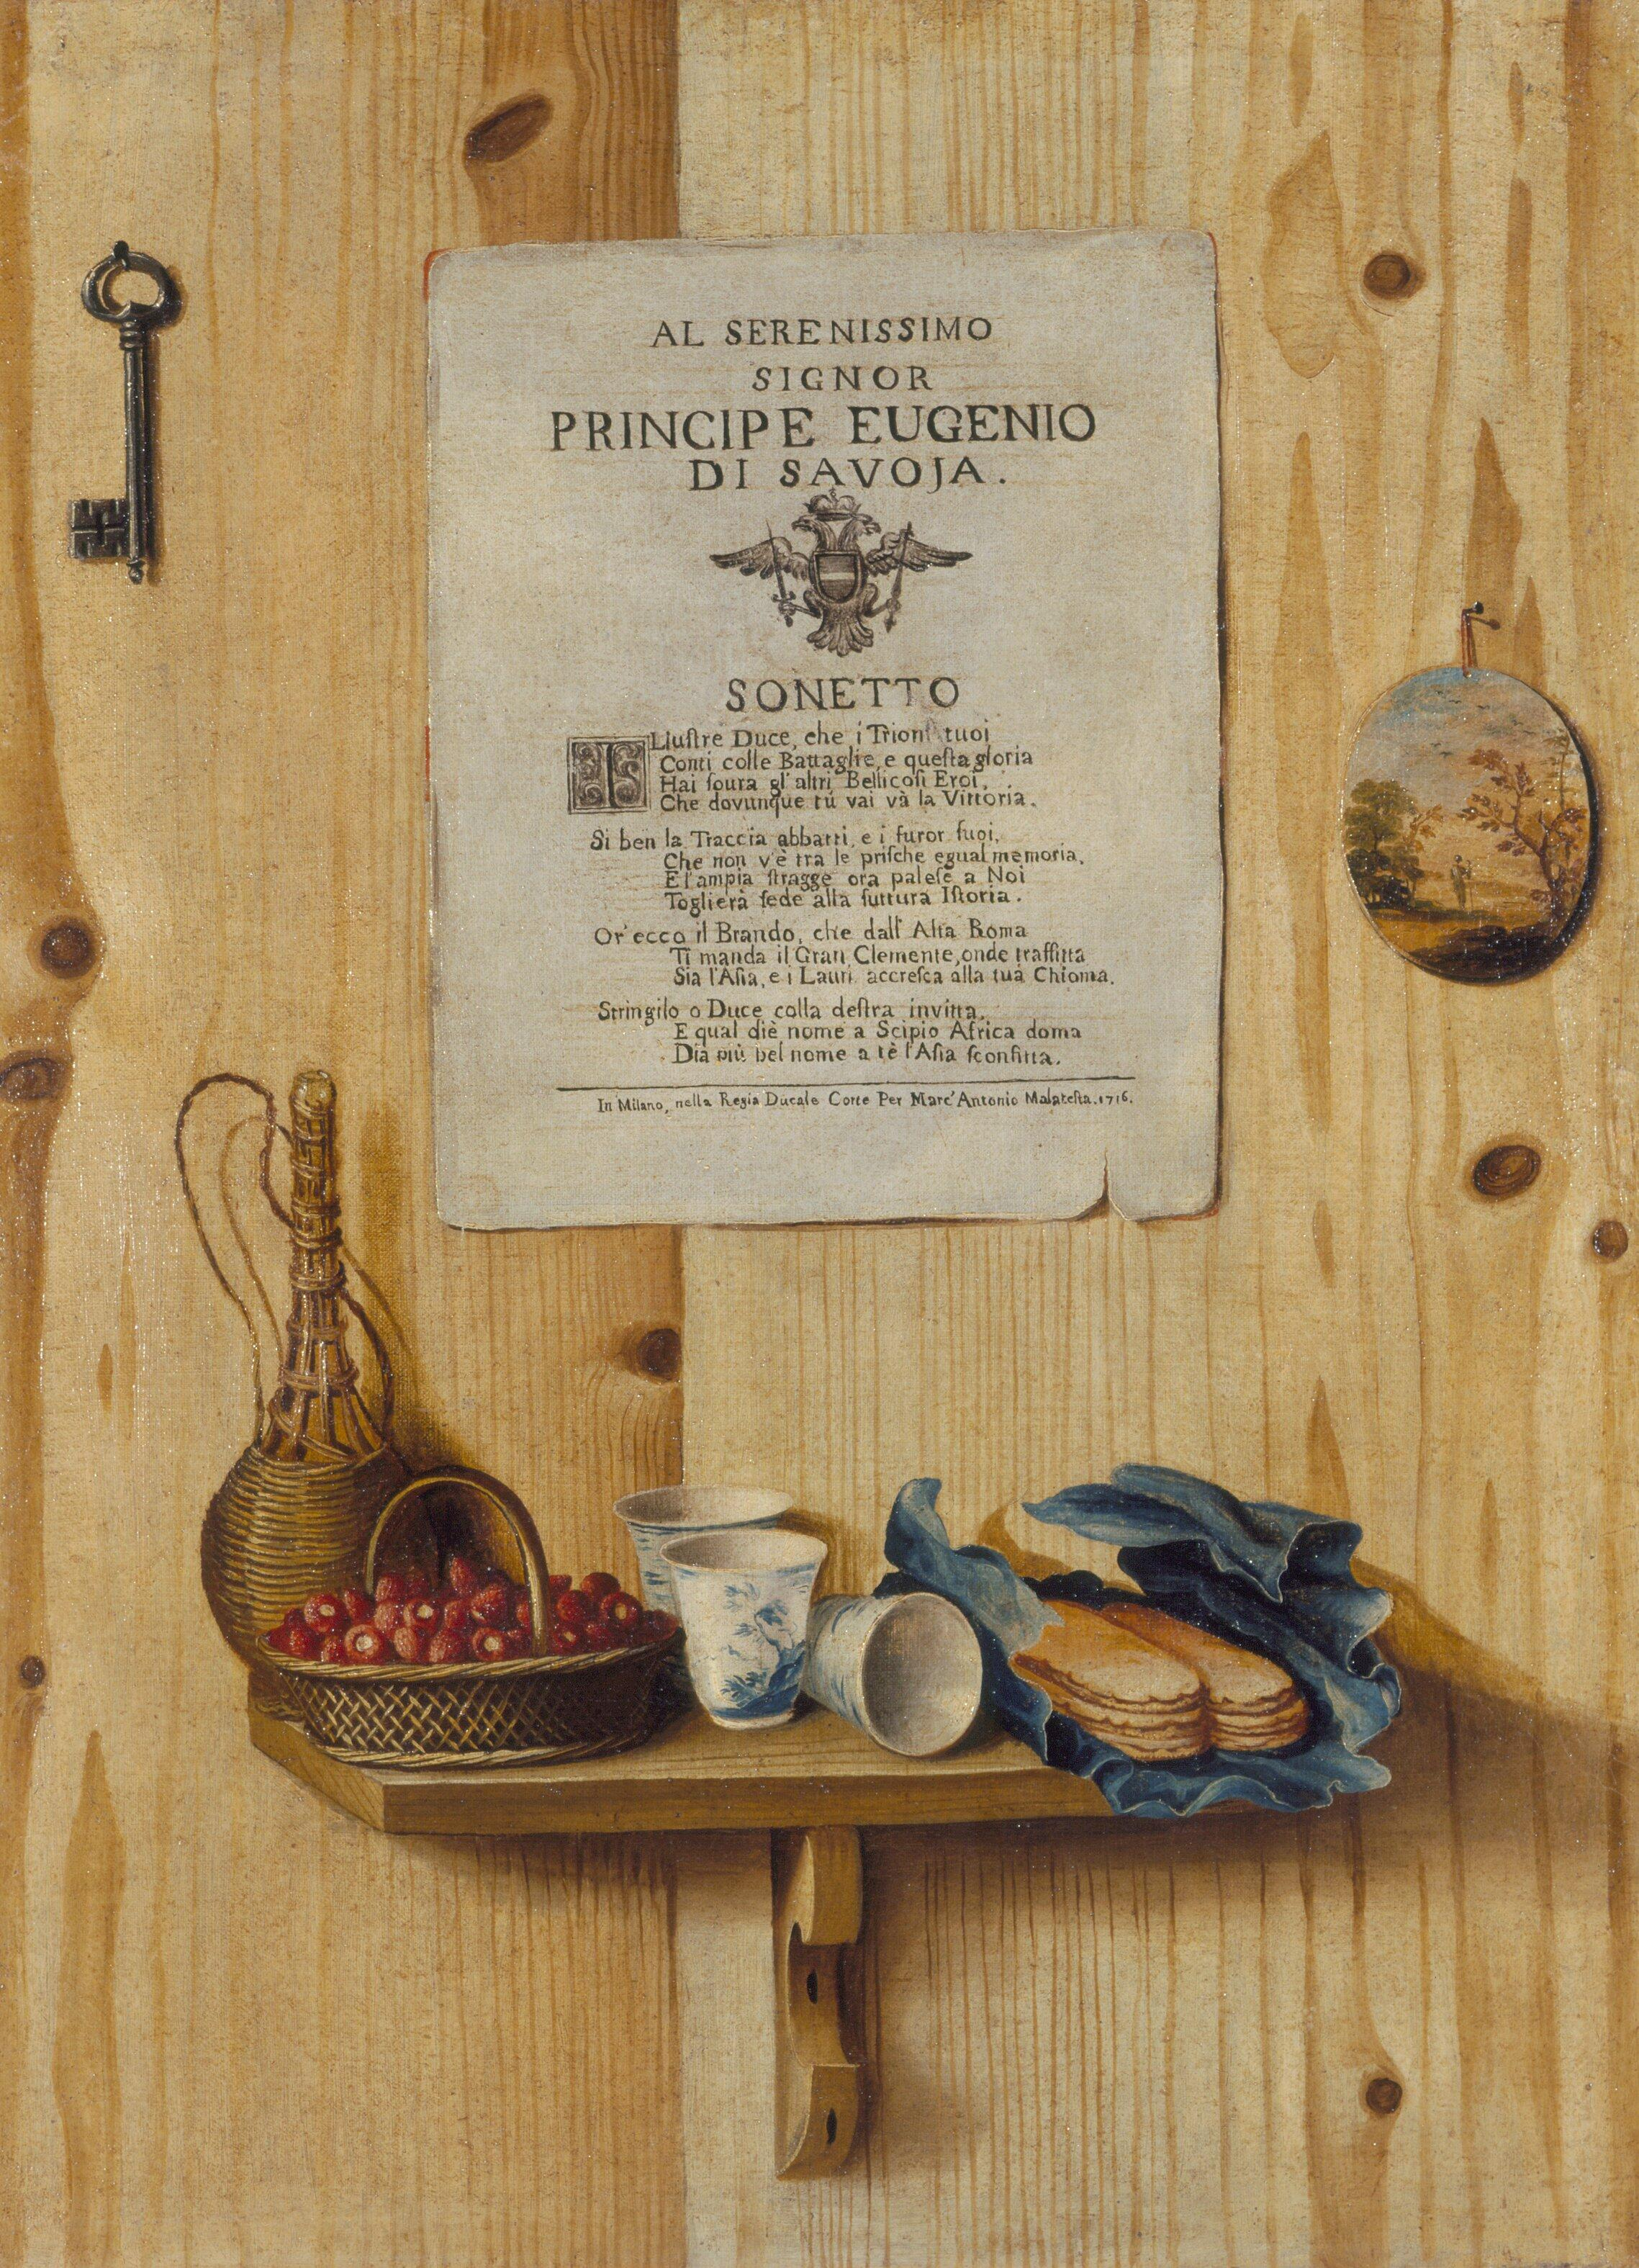
\includegraphics[scale=0.078]{Gianlisi_Antonio_Junior-Trompe_l_oeil_con_sonetto_in_onore_di_Eugenio_di_Savoia_e_mensola_con_oggetti.jpg}}
					};
				\end{tikzpicture}
				\captionsetup{labelformat=empty}
				\captionof{figure}{\hspace*{15mm}\#11}
				
			}&{
				\hspace{5mm}
				%Gianlisi Antonio Junior - Trompe l'oeil con paesaggio forbici e mensola con oggetti
				\begin{tikzpicture}
					\node[draw,dashed]
					{
						\setlength{\fboxsep}{0pt}\fbox{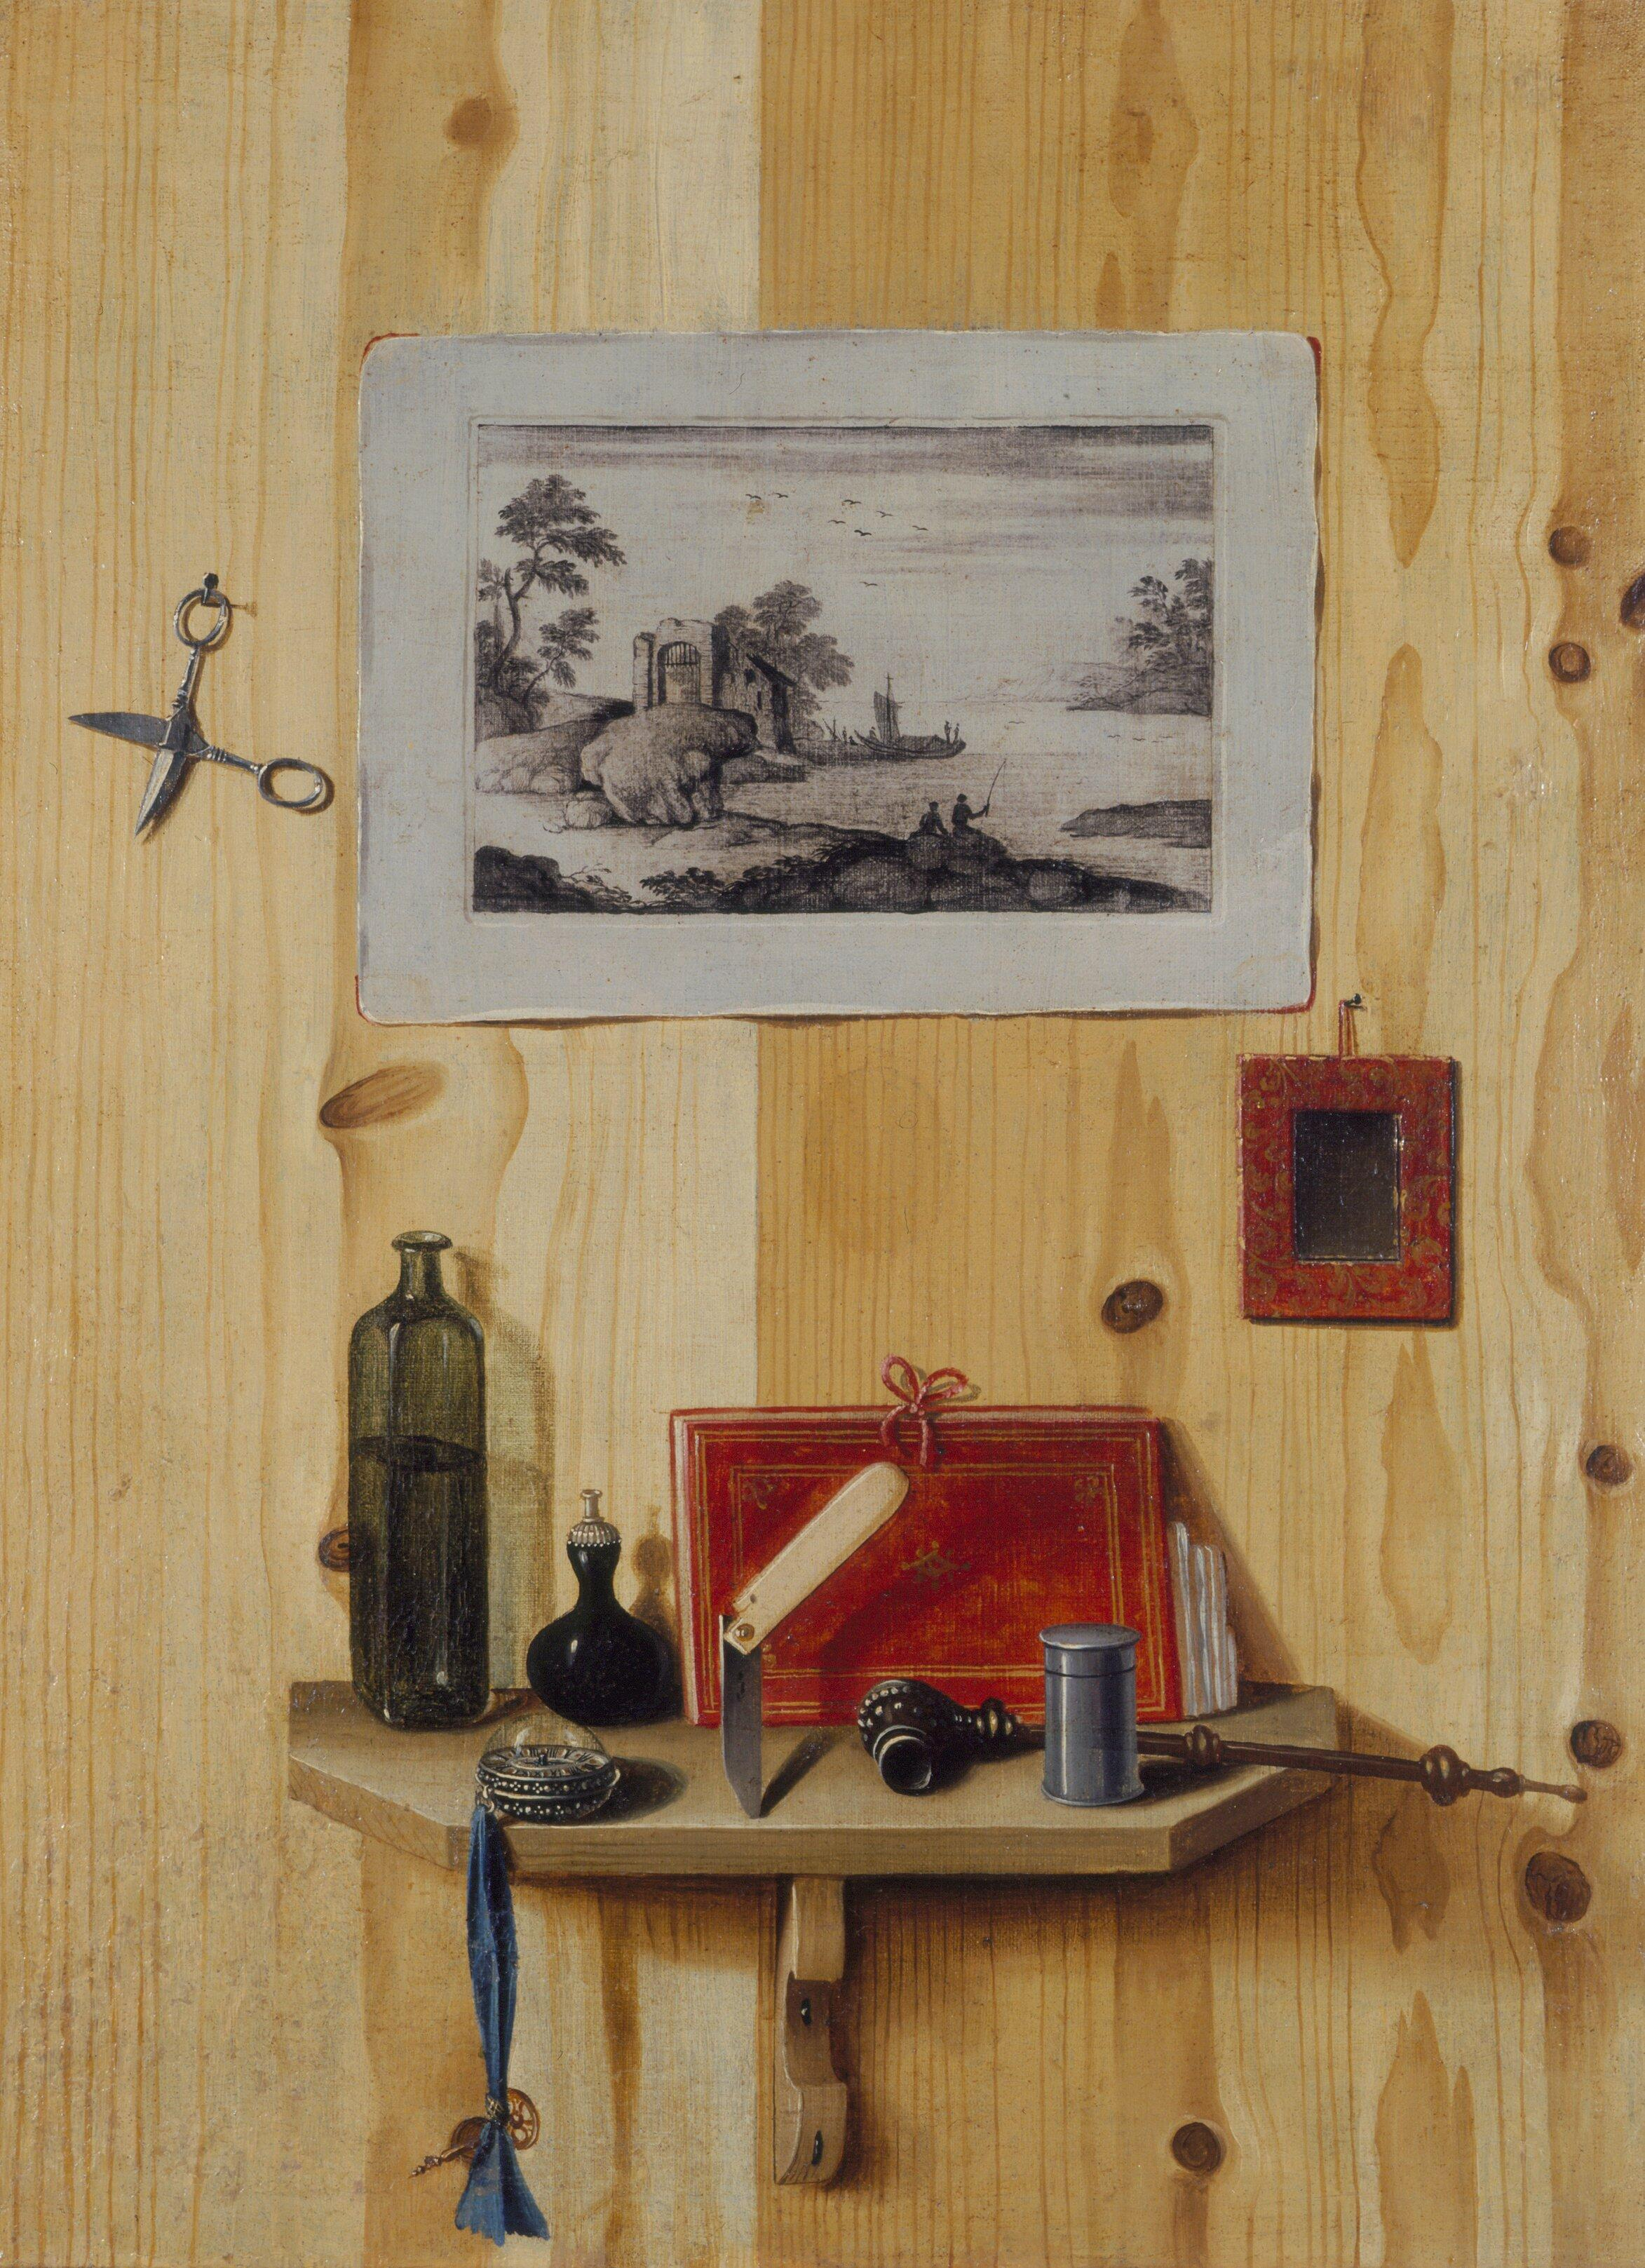
\includegraphics[scale=0.078]{Gianlisi_Antonio_Junior-Trompe_l_oeil_con_paesaggio_forbici_e_mensola_con_oggetti.jpg}}
					};
				\end{tikzpicture}
				\captionsetup{labelformat=empty}
				\captionof{figure}{\hspace*{15mm}\#12}
			}
		\end{tabularx}
	
	\newpage
	
	%--------- Page 5 ----------
	
	%First line
	\begin{tabularx}{\linewidth}{XX}
		{
			
			%Scacciani Antonio - Vassoio - Rosa
			\hspace{-40mm}
			\begin{tikzpicture}
				\node[draw,dashed]
				{
					\setlength{\fboxsep}{0pt}\fbox{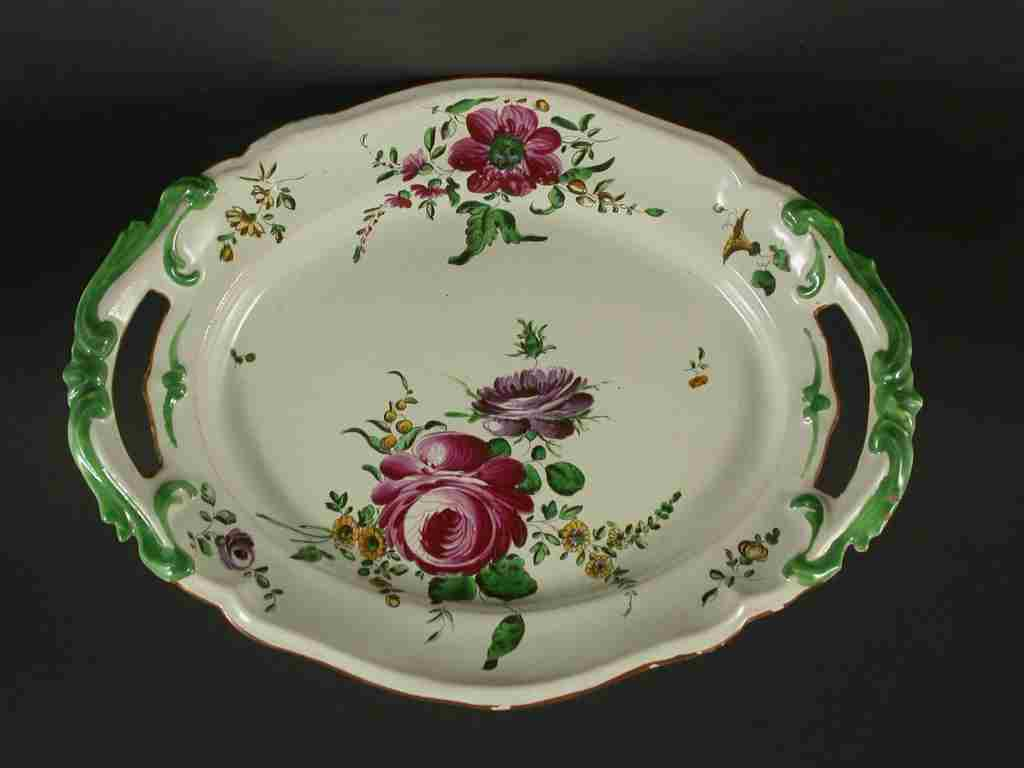
\includegraphics[scale=0.9]{Scacciani_Antonio-Vassoio-Rosa.jpg}}
				};
			\end{tikzpicture}
			\captionsetup{labelformat=empty}
			\captionof{figure}{\hspace*{-65mm}\#13}
			
			
		}&{
		
			%Realfonzo Tommaso - Natura morta con dolci frutta uova e formaggi
			\hspace{-20mm}
			\begin{tikzpicture}
				\node[draw,dashed]
				{
					\setlength{\fboxsep}{0pt}\fbox{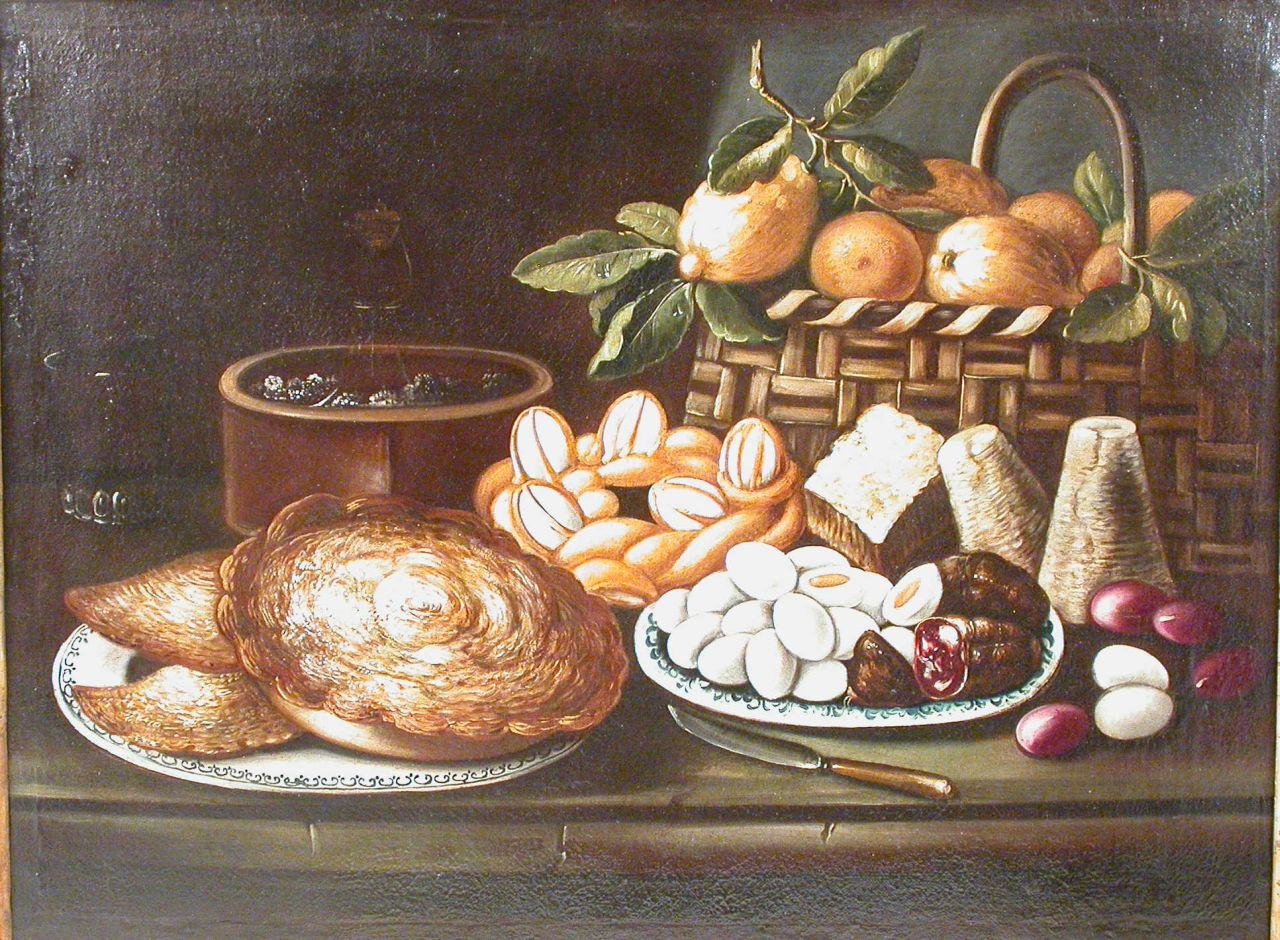
\includegraphics[scale=0.76]{Realfonzo_Tommaso-Natura_morta_con_dolci_frutta_uova_e_formaggi.jpg}}
				};
			\end{tikzpicture}
			\captionsetup{labelformat=empty}
			\captionof{figure}{\hspace*{-20mm}\#14}
			
		}
	\end{tabularx}
	
	%Second line
	\vspace{5mm}
	\nopagebreak
	\begin{tabularx}{\linewidth}{X}
		\begin{center}
			
			%Gessi Giovan Francesco - Morte di Adone
			\hspace{25mm}
			\begin{tikzpicture}
				\node[draw,dashed]
				{
					\setlength{\fboxsep}{0pt}\fbox{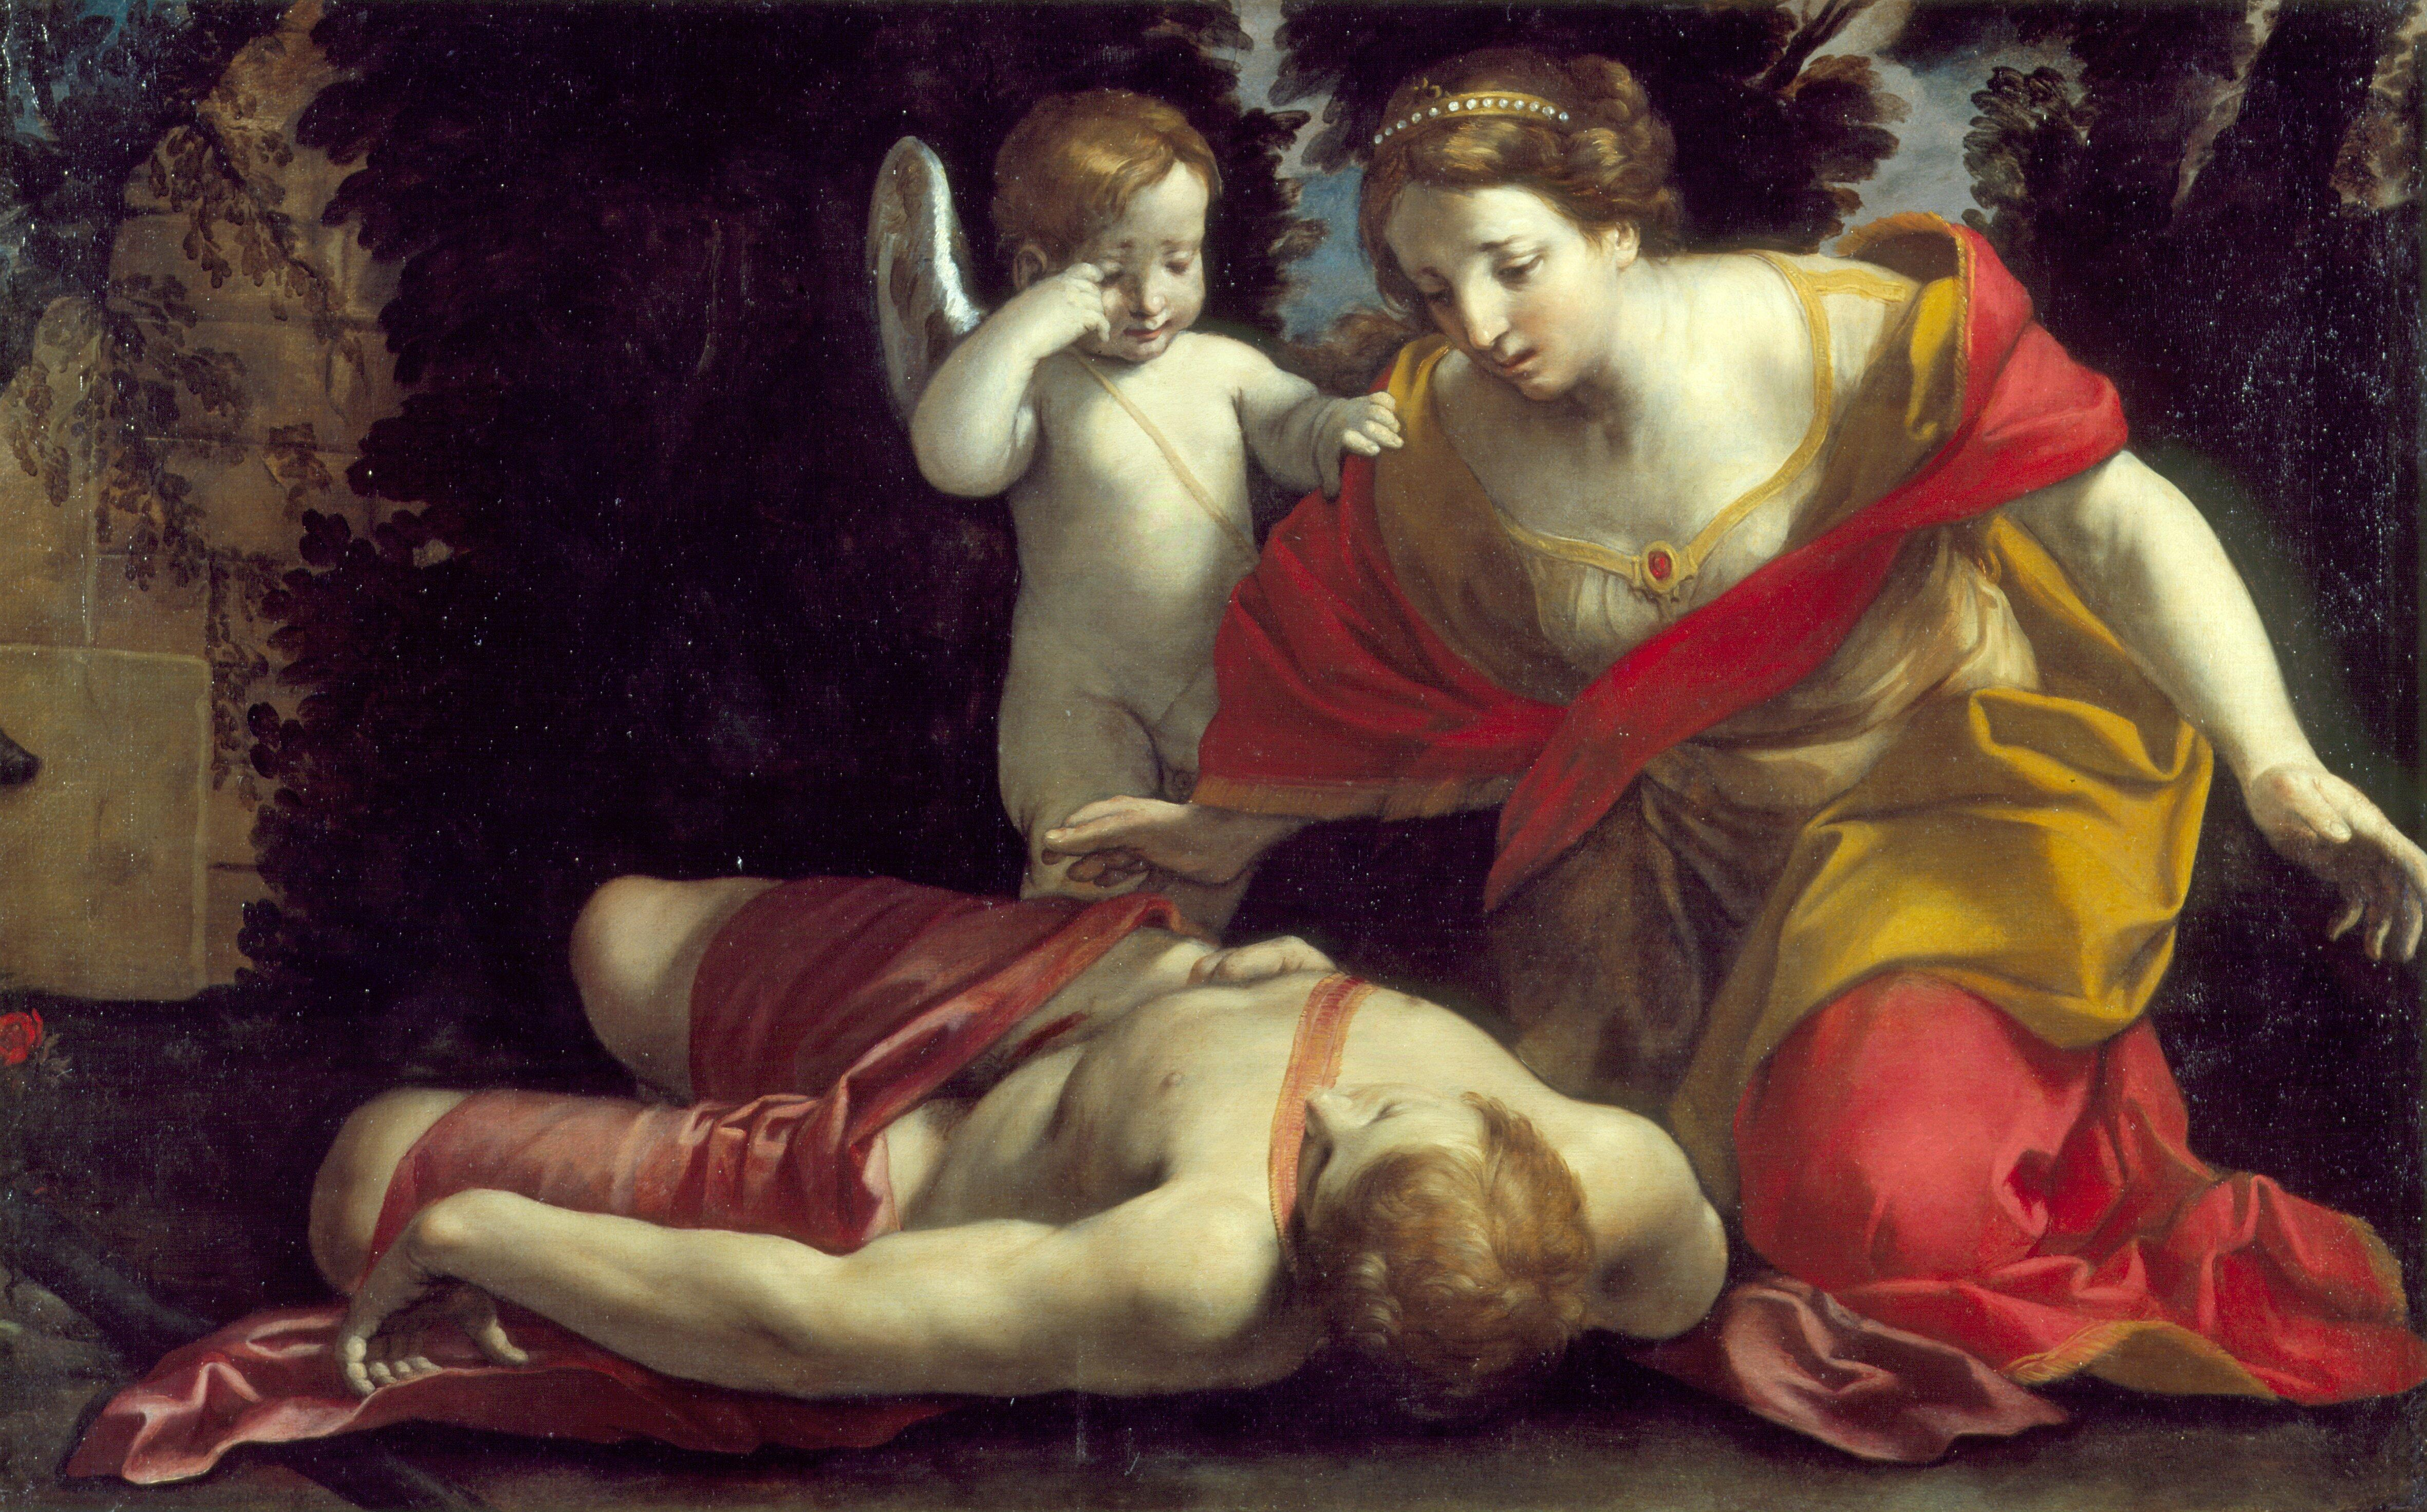
\includegraphics[scale=0.05]{Gessi_Giovan_Francesco-Morte_di_Adone.jpg}}
				};
			\end{tikzpicture}
			\captionsetup{labelformat=empty}
			\captionof{figure}{\hspace*{30mm}\#15}
			
		\end{center}
	\end{tabularx}
	
	%License
	\vspace*{\fill}
	\doclicenseThis
	
	
\end{document}